\chapter{Density Functional Theory}
	In this chapter we follow \cite{DFTWIEN2k}, \cite{DFTValenti} and \cite{DFTEngel}\\\\
	Calculating band structures and density of states a description of the coulomb interaction between electrons and ions is needed. In the past years the \textit{Hartree-Fock method} was a good way to solve calculation problems for atoms and molecules, but not for big systems as used in todays solid state physics. Due to new computational power and new numerical possibilities the \textit{density functional theory} due to P. Hohenberg and W. Kohn \cite{HohenbergKohn} has introduced new standards in solid state physics. \\\\		
	In the following chapter we will introduce the density functional theory, which is the basis of \textit{FPlO 14.00}, a software used to compute the band structures and density of states. We will start with the \textit{Hatree-Fock method} and end with the discussion of the result obtained by the density functional calculations.
	
	\section{Hartree approximation}
		In 1929 Hartree proposed that the electron system can be fully characterized by the electronic density $n_e(\vec r)$. Instead of feeling the potential of every single electron, they only feel the Coulomb potential created by the charge density $p(\vec r) = -e n_e(\vec r)$. The Coulomb potential at a point $\vec r$ is therefore given as :
		\begin{equation}
			\phi_{e-e}=(\vec r) = \frac{1}{4 \pi \epsilon_0}\int d \vec r'\frac{p(\vec r)}{|\vec r - \vec r'|} =  -\frac{e}{4 \pi \epsilon_0}\int d \vec r'\frac{n(\vec r)}{|\vec r - \vec r'|}.
		\end{equation}
		Consequently the one-particle Hartree potential
		\begin{equation}
			V_H (\vec r) = - \phi_{e-e}(\vec r) = e^2 \int d \vec r' \frac{n_e(\vec r')}{|\vec r - \vec r'|}.
		\end{equation}
		Adding the potential of the static ions (Section \ref{sec:bornOppenheimer}) obtains the total effective potential
		\begin{equation}
			\label{eq:HatreeEffectivePotential}
			V_{eff}(\vec r) = V_{ion} (\vec r) + V_H(\vec r).
		\end{equation}
		We now want to find an expression for the density $n(\vec r)$, which is given as the sum of all electrons at a point $\vec r$
		\begin{equation}
			n(\vec r) = \sum_{i=1}^{N_e} \delta(\vec{r - r_i}).
		\end{equation}
		Thus we can calculate the expectation value of the density
		\begin{equation}
			\label{eq:densityExpectation}
			n_e(\vec r) = \langle \psi | n(\vec r) | \psi \rangle = \langle \psi | \sum_{i=1}^{N_e} \delta(\vec{r - r_i}) | \psi \rangle.
		\end{equation}
		In the Hartree approximation the complete Hamiltonian is only the sum over all energies of the single electrons. Consequently it assumes, that the many-body wave function $\psi$ is written as a product of the wave function of the occupied single-particle states,
		\begin{equation}
			\psi = \phi_{\lambda_1, \sigma_1}(\vec r_1, s_1)\phi_{\lambda_2, \sigma_2}(\vec r_2, s2) \dots \phi_{\lambda_{N_e}, \sigma_{N_e}}(\vec r_{N_e}, s_{N_e}) 
		\end{equation}
		We used the quantum number $\lambda$ in the last equation, that stands for the wave vector $\vec k$ and the band index n. Plugging the above expression into the density expectation value (Eq. \ref{eq:densityExpectation})
		we have
		\begin{equation}
			\begin{split}
				n_e(\vec r) &= \sum_{i=1}^{N_e} \int d\vec r_1 \int d s_1 \int d \vec r_2 \int d s_2 \dots \int \vec r_{N_e} \int s_{N_e} \\ & \cdot \phi_{\lambda_1, \sigma_1}^*(\vec r_1, s_1) \phi_{\lambda_2, \sigma_2}^*(\vec r_2, s_2) \dots \phi_{\lambda_{N_e}, \sigma_{N_e}}^*(\vec r_{N_e}, s_{N_e}) \\ & \cdot \delta(\vec{r - r_i}) \phi_{\lambda_1, \sigma_1}^*(\vec r_1, s_1)\phi_{\lambda_2, \sigma_2}^*(\vec r_2, s_2) \dots \phi_{\lambda_{N_e}, \sigma_{N_e}}^*(\vec r_{N_e}, s_{N_e}) \\
				&= \sum_{i=1}{N_e} |\phi_{\lambda_i}(\vec r)|^2.
			\end{split}
		\end{equation}
		From the single particle Hamiltonian with the effective potential (Eq. \ref{eq:HatreeEffectivePotential})
		\begin{equation}
			\hat H = - \frac{\hbar^2}{2 m_e} \nabla^2 \phi_{\lambda_i} (\vec r) + V_{ion} + e^2 \sum_{i \neq j}^{N_e} \int d \vec r' \frac{n(\vec r')}{|\vec{r - r'}|},
		\end{equation}
		we get the \textit{Hartree equations} :
		\begin{equation}
			- \frac{\hbar^2}{2 m_e} \nabla^2 \phi_{\lambda_i} (\vec r) + V_{ion} + e^2 \sum_{i \neq j}^{N_e} \int d \vec r' \frac{|\phi_{\lambda_i}(\vec r')|^2}{|\vec{r - r'}|} = \epsilon_{\lambda_i} \phi_{\lambda_i} (\vec r)
		\end{equation}
		which can be written as 
		\begin{equation}
			- \frac{\hbar^2}{2 m_e} \nabla^2 \phi_{\lambda_i} (\vec r) + V_{ion} + e^2 \sum_{i \neq j}^{N_e} \int d \vec r' U(\vec{r - r'})|\phi_{\lambda_i}(\vec r')|^2 \phi_{\lambda_i}(\vec r) = \epsilon_{\lambda_i} \phi_{\lambda_i} (\vec r)
		\end{equation}
		for a general two-particle interaction. Notice that the \textit{Hatree equations} are not consistent with the \textit{Pauli exclusion principle}, which states that two identical fermions (electrons) cannot occupy the same quantum state simultaneously. Consequently we have to introduce the \textit{Slater Determinant} and the \textit{Hartree-Fock equations}. 
		
		
		
	
	\section{Hartree-Fock approximation}
		Due to the \textit{Pauli principle} the total electronic wave function has to be completely antisymmetric.
		\begin{equation}
			\psi(..., \vec r_i, s_i, ..., \vec r_j, s_j, ...) = 	- \psi(\dots, \vec r_j, s_j,  \dots, \vec r_i, s_i, \dots) 
		\end{equation}
		The so-called \textit{Slater determinant} satisfies the antisymmetric requirement,
		\begin{equation}
			\Psi_{HF} = \frac{1}{\sqrt{N_e !}} 
			\begin{vmatrix}
				\phi_{\lambda_1, \sigma_1} (\vec r_1, s_1) & \phi_{\lambda_1, \sigma_1} (\vec r_2, s_2) & \dots & \phi_{\lambda_1, \sigma_1} (\vec r_{N_e}, s_{N_e}) \\
				\phi_{\lambda_2, \sigma_2} (\vec r_1, s_1) & \phi_{\lambda_2, \sigma_2} (\vec r_2, s_2) & \dots & \phi_{\lambda_2, \sigma_2} (\vec r_{N_e}, s_{N_e}) \\
				\vdots & \vdots & \ddots & \vdots \\
				\phi_{\lambda_{N_e}, \sigma_{N_e}} (\vec r_1, s_1) & \phi_{\lambda_{N_e}, \sigma_{N_e}} (\vec r_2, s_2) & \dots & \phi_{\lambda_{N_e}, \sigma_{N_e}} (\vec r_{N_e}, s_{N_e})
			\end{vmatrix}
		\end{equation}
		With the the introduced wave function $\psi_{HF}$ we can evaluate the expectation value :
		\begin{equation}
			\begin{split}
				E_{HF} = \langle H \rangle =& \sum_{i=1}^{N_e} \int d \vec r \phi_{\lambda_i}^*(\vec r) [- \frac{\hbar ^2}{2m_e} \nabla^2 + V_{ion}(\vec r)] \phi_{\lambda_i}(\vec r) \\ &+ \frac{e^2}{2} \sum_{i,j =1}^{N_e} \int d \vec r \int d \vec r' \frac{|\phi_{\lambda_j}(\vec r')|^2}{|\vec{r - r'}|} |\phi_{\lambda_i}(\vec r)|^2 \\
				&- \frac{e^2}{2} \sum_{i,j = 1}^{N_e} \int d \vec r \int d \vec r' \frac{1}{|\vec{r - r'}|} \delta_{\sigma_i, \sigma_j} \phi_{\lambda_i}^*(\vec r) \phi_{\lambda_j}^*(\vec r')\phi_{\lambda_i}(\vec r') \phi_{\lambda_j}(\vec r) 
			\end{split}
		\end{equation}
		Independent variation finally leads to the \textit{Hartree-Fock equations}.
		\begin{equation}
			\begin{split}
				-\frac{\hbar^2}{2m_e} \nabla^2 \phi_{\lambda_i(\vec r)} + & V_{ion}(\vec r) \phi_{\lambda_i}(\vec r) + e^2 \sum_{j=1}^{N_e} \int d \vec r' \frac{|\phi_{\lambda_j}(\vec r')|^2}{|\vec{r -r'}|} \phi_{\lambda_i}(\vec r) \\ &
				- e^2 \sum_{j=1}^{N_e} \int d \vec r' \frac{\phi_{\lambda_j}^*(\vec r') \phi_{\lambda_i}(\vec r')}{|\vec{r - r'}|}\phi_{\lambda_j}(\vec r) \delta_{\sigma_i, \sigma_j} = \epsilon_{\lambda_i} \phi_{\lambda_i}(\vec r)
			\end{split}
		\end{equation}
		The above equation can also be rewritten for a general two-particle interaction :
		\begin{equation}
			\begin{split}
				- \frac{\hbar^2}{2m_e} \nabla^2 & \phi_{\lambda_i}(\vec r) + V_{ion}(\vec r)\phi_{\lambda_i}(\vec r) + \sum_{j=1}^{N_e} \int d \vec r' U(\vec{r - r'}) |\phi_{\lambda_j(\vec r')|^2 \phi_{\lambda_i}} \\ & - \sum_{j=1}^{N_e} \int d \vec r' U(\vec{r - r'})\phi_{\lambda_j}^*(\vec r') \phi_{\lambda_i}(\vec r') \phi_{\lambda_j}(\vec r) \delta_{\sigma_i, \sigma_j} = \epsilon_{\lambda_i} \phi_{\lambda_i}(\vec r)
			\end{split}
		\end{equation}	
		With the \textit{Hartree method} in mind we now want to continue with the \textit{density functional theory}, which is based on the two theorems postulated by Hohenberg and Kohn \cite{HohenbergKohn}.
	
	\section{Hohenberg-Kohn Theorems}
		The two theorems are fundamental for modern density functional calculations and will show us that a system can be fully characterized by its ground- state density.
	
		\subsection*{Theorem 1}
			There is a one-to-one correspondence between $V_{ext}(\vec{r})$ and the ground state density $n_0$. 
			\begin{equation}
				V_{ext}(\vec{r}) \Leftrightarrow |\psi_0 \rangle \Leftrightarrow n_0(\vec{r})
			\end{equation}
		
		\subsection*{Theorem 2}
			Any measurable property O of our system can now be written as a functional of the state density
			\begin{equation}
				O[n] := \langle \psi[n] | \hat O | \psi[n] \rangle,
			\end{equation}
			leading to the energy
			\begin{equation}
				E[n] = \langle \psi[n] | \hat H | \psi[n] \rangle = F_{HK}[n] + \int d^3 r V_{ext}(\vec{r}) n(\vec{r}) 
				\label{eq:EnergyFunctional}
			\end{equation}
			with $F_{HK}$ as Hohenberg-Kohn functional denoted as :
			\begin{equation}
				F_{HK}[n] := \langle \psi[n] | \hat T + \hat U | \psi[n] \rangle
			\end{equation}	
		We are not proofing the theorems (proofs given in \cite{ElectronicStructureBook}), but we want to discuss the fundamental meaning of them. \\\\
		Regarding an arbitrary many body system having a unique external potential $V_{ext}$, we also have a unique ground state many particle wave function $\psi_0$. The many particle wave function by itself leads to the ground- state density $n_0$, which contains according to the first theorem all observables. \\\\
		We also have to mention the universality of $F_{HK}[n]$. Supposing that the ground state density is known we can calculate the contribution of the external potential $V_{ext}$. In addition $F_{HK}$ does not contain any information about the nuclei and their position. Consequently $F_{HK}$ represents a \textbf{universal function} for an many-electron system. \\\\
		Due to the second theorem one can finally find the ground state density by using the variational principle of \textit{Rayleigh Ritz}.\\\\
		In general, because of the complexity of the difficult many-body Hamiltonian, we cannot obtain the ground state density. Thus we need to change into a different auxiliary system with the \textit{Kohn Sham approach}.			

	\section{The Kohn-Sham ansatz}
		The \textit{Kohn-Sham equations} were published in 1965 right after the \textit{Hohenberg Kohn theorems}, by W. Kohn and L. J. Sham in \cite{KohnSham} and are used as a practical tool to calculate the ground state density. Kohn and Sham assumed that the ground state density of the original system is equal to the ground state density of some chosen non-interacting systems. This leads to independent-particle equations for non-interacting systems, while putting all the difficult many-body terms into an \textit{exchange correlation potential}.\\
		Splitting the many-body Hamiltonian from Equation  \ref{eq:generalHamiltonian} into single-particle Hamiltonians we have 
		\begin{equation}
			H_s = - \frac{1}{2} \sum_i \nabla_r^2 + \sum_i v_s.
		\end{equation} 
		$H_s$ describes a non-interacting system, which yields the ground state energy. For a non-interacting system one can obtain the ground state density by solving the one-particle Schrödinger equation. Therefore we rewrite Equation \ref{eq:EnergyFunctional} into 
		\begin{equation}
			E_{KS}[n] = T_s + E_H[n] + E_{ext}[n] + E_{xc},
		\end{equation}
		where the independent-particle kinetic energy $T_s$ is given by 
		\begin{equation}
			\label{eq:KohnShamKineticEnergy}
			T_s = - \frac{1 }{2} \sum_{\sigma}\sum_{i=1}^{N} \langle \psi_i(\vec r) | \nabla^2 | \psi_i(\vec r) \rangle.
		\end{equation}
		The classical Coulomb interacting energy (Hartree energy $E_H$) is defined by
		\begin{equation}
			E_H[n] = \frac{1}{2} \int d^3r d^3r' \frac{n(\vec r) n(\vec r')}{|\vec r - \vec r'|}. 
		\end{equation}
		Integrating over the external potential multiplied by the density we have
		\begin{equation}
			E_{ext} = \int d\vec r  v_{ext}(\vec r)n(\vec r).
		\end{equation}
		Finally the missing exchange-correlation energy $E_{xc}$ groups all the many-body effects on the independent particle and will be discussed in section \ref{sec:TheExchangeCorrelationEnergy}. We just want to mention here, that the accuracy of the Kohn-Sham approach is in general exact and only depends on the precision of the exchange correlation potential.\\\\
		The Kohn-Sham results from a minimization of the total energy by a variation of the density. By varying the wave functions and using the chain rule we get the variational equation.
		\begin{equation}
			\label{eq:KohnShamVariationalEquation}
			\frac{\delta E_{KS}[n]}{\delta \psi_i(\vec r)} = \frac{\delta T_s}{\delta \psi_i(\vec r)} + \left[ \frac{\delta E_H}{\delta n(\vec r)} + \frac{\delta E_{ext}}{\delta n(\vec r)} + \frac{\delta E_{xc}}{\delta n(\vec r)} \right] \frac{\delta n(\vec r)}{ \delta \psi_i(\vec r)}
		\end{equation}
		Considering orthogonal wave vectors
		\begin{equation}
			\langle \psi_i | \psi_j \rangle = \delta_{ij},
		\end{equation}
		and the normalization
		\begin{equation}
			\label{eq:KohnShamSecondOrderCondition}
			n(\vec r) = \sum_{i=1}^{N}|\psi_i (\vec r)|^2,
		\end{equation}
		the single kinetic energy and the density can be expressed as :
		\begin{subequations}
			\begin{align}
				\frac{\delta T_s}{\delta \psi_i (\vec r)} &= - \frac{\hbar^2}{2m} \nabla^2 \psi_i (\vec r),\\
			    \frac{\delta n(\vec r)}{\delta \psi_i(\vec r)} &= \psi_i (\vec r).
			\end{align}
		\end{subequations}	
		Due to the orthogonality relation the sums vanishes. Additionally the derivation of the ground state density turns into the $i^{th}$ wave function $\psi_i(\vec r)$. The derivations of the remaining energies become the corresponding potentials. Thus the Hamiltonian can be written as : 
		\begin{equation}
			H_{KS} = -\frac{1}{2} \nabla^2 + v_{H} + v_{ext} + v_{xc}
		\end{equation}
		Due to the second-order condition \ref{eq:KohnShamSecondOrderCondition} we use the Lagrange Multiplier method to minimize the density and get the \textit{Kohn-Sham Schrödinger-like} equations
		\begin{equation}
			\label{eq:KohnShamLagrangeMethod}
			(H_{KS} - \epsilon_i)\Psi_i(\vec r) = 0,
		\end{equation}
		or detailed 
		\begin{equation}
			\left[ - \frac{1}{2} \nabla_\vec r^2 + v_{ext} + \int d\vec r' \frac{n(\vec r')}{|\vec r - \vec r'|} + v_{xc} \right] \psi_i (\vec r) = \epsilon_i \psi_i (\vec r),
		\end{equation}
		where $\epsilon_i$ is the Lagrange multiplier and the eigenvalue of $H_{KS}$ (the energy of the single particle). \\\\
		Equation \ref{eq:KohnShamLagrangeMethod} is an eigenvalue problem which depends on a potential that must be found self-consistently. The last missing part for an iterative solution is the missing \textit{exchange correlation potential}, which we will obtain in the following section.
		
	\section{The exchange-correlation energy}
	\label{sec:TheExchangeCorrelationEnergy}
		As we are using the \textit{general-gradient approximation} we will describe both, the \textit{local-density approximation} and the \textit{general-gradient approximation} within this chapter.
		\subsection{Local-density approximation (LDA)}
			The oldest and for decades most used density functional theory application is the \textit{Local-density approximation}, which approximates the exchange-correlation-energy density of inhomogeneous systems locally by the exchange-correlation-energy  density of an homogeneous electron gas for infinitesimal small volumes and slowly changing electronic densities. 
			\begin{equation}
				E_{xc-LDA}[n] = \int \epsilon_{xc-LDA}(n) n(\vec r) d \vec r
			\end{equation}
			An advantage of the \textit{Local-density approximation} is its simple utilization in \textit{Kohn-Sham equations} as corresponding exchange-potential.
			\begin{equation}
				V_{xc-LDA}(\vec r) = \frac{\delta \epsilon_{xc-LDA}[n]}{\delta n(\vec r)} = \int d^3 \vec r'\frac{d \epsilon_{xc}(n)}{dn}\big|_{n=n(\vec r')} \frac{\delta n(\vec r')}{\delta n(\vec r)} = \frac{d \epsilon_{xc} (n)}{d n}\big|_{n=n(\vec r)}
			\end{equation}
			The exchange component is given by:
			\begin{equation}
				V_{x-LDA} (\vec r) = - \frac{(3\pi^3)^\frac{1}{3}}{\pi}e^2n^\frac{1}{3}(\vec r),
			\end{equation}
			whereas the correlation component can be calculated from  quantum Monte-Carlo methods. \\\\
			The advantage of the local density approximation is its simplicity as well as the good  results it yields for valid systems. FTo solve other systems and to improve the accuracy there are different methods like the \textbf{local-spin-density approximation}, which includes the magnetization density $m(\vec r) = n_\uparrow (\vec r) - n_\downarrow (\vec r)$, where $\sigma = \uparrow, \downarrow$ represents the spin direction. With the \textit{local-spin-density approximation} it is now possible to distinguish between ferromagnetic and anti-ferromagnetic ground states. The exchange-correlation is given as
			\begin{equation}
				E_{xc-LSDA}[n_\uparrow, n_\downarrow] = \int E_{xc-LSDA}(n_\uparrow(\vec r), n_\downarrow(\vec r))n(\vec r)d \vec r,
			\end{equation}
			with the electron density $n(\vec r) = n_\uparrow (\vec r) + n_\downarrow (\vec r)$. \\\\
			Another improvement of the local-spin-density approximation is the \textbf{generalized-gradient approximation}, which is used in our calculations.
		\subsection{Generalized-gradient approximations (GGA)}
			In the \textit{general-gradient approximation} the neighboring volumes also contribute in terms of a density gradient, unlike in the \textit{local-density approximation}, where only the single volume densities were used. There are different possibilities to define such a gradient. Some uses experimental data, which excludes the ab-initio advantages of the density functional theory, while others do not. The accuracy of the general-gradient approximation varies from system to system and has to be chosen individually. The exchange-correlation energy is now given as :
			\begin{equation}
				\begin{split}
					E_{xc-GGA}[n_\uparrow, n_\downarrow] &= \int \epsilon_{xc-GGA} (n_\uparrow(\vec r), n_\downarrow(\vec r), |\nabla n_\uparrow|, |\nabla n_\downarrow|)n(\vec r)d\vec r \\
					&= \int \epsilon_{xc-hom}(n)F_{GGA} (n_\uparrow(\vec r), n_\downarrow(\vec r), |\nabla n_\uparrow|, | \nabla n_\downarrow|) n(\vec r) d \vec r.
				\end{split}
			\end{equation}
	
	\section{Solving the Kohn-Sham equations}
		After introducing the \textit{Kohn-Sham equations} we ended up with an infinite system of single particle equations.
		\begin{equation}
			\hat H_{sp} \psi_i (\vec r) = \left[ - \frac{\hbar^2}{2m} \nabla_\vec r^2 \underbrace{v_{ext}(\vec r) + \frac{e^2}{4 \pi \epsilon_0} \int d \vec r'\frac{n(\vec r')}{| \vec r - \vec r'|} + v_{\alpha}}_{v_{eff}} \right] \psi_i (\vec r) = \epsilon_i \psi_i (\vec r)
		\end{equation}
		with $v_\alpha$ as the chosen exchange-correlation potential form the previous section. \\
		$\psi_i$ can be expanded as linear combination of an arbitrary basis $\psi_p^b$
		\begin{equation}
			\psi_i(\vec r) = \sum_{p=1}^{P} c_p^{\vec k n} \psi_p^{b},
		\end{equation}
		where $\psi_i (\vec r)$ belongs to a function space with an infinite dimension. Consequently we have an infinite integer P. However, as we are performing our calculations with computers P must be limited. \\\\
		Furthermore we need to acknowledge what a good basis consists of. If a basis set is very similar to $\psi_i$ we require only a small set of wave functions. The basis set is therefore called \textit{efficient}. However in general we do have to know the solution before performing the calculations to obtain an \textit{efficient} basis set. In most cases the required P is much higher than what is affordable. Limiting P leads to $\psi_p^{\vec k n}$ wave functions, which have to carry many properties and are 'specialized' to a certain system. These wave functions are called \textit{biased}. For a good basis set we want to have an \textit{efficient} and \textit{unbiased} set of basis vectors. \\\\
		Having chosen a basis the expanded \textit{Kohn-Sham equations} turn into an eigenvalue problem with P-eigenvalues :
		\begin{equation}
			\label{eq:KohnSahmEigenvalueProblem}
			\begin{pmatrix}
				\dots & \dots & \dots \\
				\vdots & \langle \psi_i^b | \hat H_{sp} | \psi_j^b \rangle - \epsilon_m \langle \psi_i^b | \psi_j^b \rangle & \vdots \\
				\dots & \dots & \dots 
			\end{pmatrix}
			\begin{pmatrix}
				c_1^{\vec k n} \\
				\vdots \\
				c_P^{\vec k n}
			\end{pmatrix}
			= \begin{pmatrix}
				0 \\
				\vdots \\
				0
			\end{pmatrix}.
		\end{equation}
		In brief we have to guess a propitiate particle density $n_0(\vec r)$, determine the effective potential $v_{eff}$ and solve the eigenvalue problem in Equation in \ref{eq:KohnSahmEigenvalueProblem}, which will give the Kohn-Sham eigenfunctions $\psi_i(\vec r)$. Then we are going to calculate a new particle density $n(\vec r)$ from the Kohn-Sham eigenfunctions $\psi_i(\vec r)$ and compare it to the old particle density $n_0 (\vec r)$. If $n(\vec r)$ does not coincide with n0(r) with satisfying accuracy the procedure is repeated till $n(\vec r)$ converged. With the first theorem of Hohenberg-Kohn it is now possible to obtain all needed properties of our solid state. \\\\
		In the next section we will derive the basis set, where our calculation software \textit{FPLO14.00} is used. 
		
		
	\section{Basis set}
		After the implementation of the exchange-correlation energy we now need a basis $\Psi$ to solve the self consistent Kohn-Sham equation. According to the Fourier theorem every periodic function can be evolved as a sum of a new function weighted with a factor
		\begin{equation}
			\psi(\vec r)_m = \sum_{n=-\infty}^{\infty} c_n^m \phi_n(\vec r).
		\end{equation}
		Consequently we have to choose a proper basis set $\phi$ and calculate the weighting factors $c_n$. The easiest basis is given by plane waves, which are the solution of the Hamiltonian of free electrons. For a more efficient but complex basis one chooses local orbitals.
		
		
		\subsection{Plane waves (PW)}
			Choosing $\phi_\vec k^n(\vec r)$ as a plane wave, we get :
			\begin{equation}
				\psi_\vec k^n(\vec r) = \sum_{\vec K} c_\vec K^{n, \vec k} e^{i(\vec k + \vec K)\vec r}.
			\end{equation}
			One basis function is therefore :
			\begin{equation}
				\phi_\vec K^\vec k (\vec r) = e^{i(\vec k + \vec K) \vec r}.
v			\end{equation}
			Because one cannot calculate a sum over the whole $\vec K$ space one have to define a maximum value $K_{max}$, which approximated the basis. $K_{max}$ is moreover often represented as the \textit{cut-off energy} :
			\begin{equation}
				E_{cut} = \frac{\hbar^2 K_{max}^2}{2m_e}.
			\end{equation}
			In addition plane waves are orthogonal, which simplifies the eigenvalue problem. \\\\
			This is the mathematically simplest form of a basis set. But it collapses for strongly bound electrons near the cores, for which it offers to use local orbitals.
			
		\subsection{Local Orbitals (LO)} 
			In this section we follow \cite{DJG01}. \\\\
			Local orbitals are solutions of the spherical symmetric Schrödinger equation and can therefore be written as spherical harmonics. Moreover this section will be helpful for a better understanding of the quantum numbers l and m. We will start with the \textit{separation of variables} of the wave function in spherical coordinates. The Laplacian takes the form :
			\begin{equation}
				\nabla^2 = \frac{1}{r^2} \left(r^2 \frac{\partial}{\partial r}\right) + \frac{1}{r^2 sin \theta} \left(\frac{\partial^2}{\partial \phi^2} \right).
			\end{equation}
			The time-independent Schrödinger equation then reads 
			\begin{equation}
				\label{eq:sphericalSchroedinger}
				-\frac{\hbar^2}{2m} \left[ \frac{1}{r^2} \left(r^2 \frac{\partial \psi}{\partial r}\right) + \frac{1}{r^2 sin \theta} \left(\frac{\partial^2 \psi}{\partial \phi^2} \right) \right] + V \psi = E \psi.
			\end{equation}
			Now we separate the wave function into a radial and an angular part.
			\begin{equation}
				\psi (r, \theta, \phi) = R(r) Y(\theta, \phi)
			\end{equation}
			Putting into Equation \ref{eq:sphericalSchroedinger} we have
			\begin{equation}
				-\frac{\hbar^2}{2m} \left[ \frac{1}{R} \left( r^2 \frac{d R}{d r}  \right) + \frac{R}{r^2 \sin \theta} \frac{\partial}{\partial \theta} \left( \sin \theta \frac{\partial Y}{\partial \phi} \right) + \frac{R}{r^2 \sin^2 \theta} \frac{\partial Y}{\partial \phi^2} \right] + VRY  = ERY	
			\end{equation}
			Dividing by RY and multiplying by $\frac{-2mr^2}{\hbar^2}$ gives us 			
			\begin{equation}
				\label{eq:schrödingerSeparated}
				\left\{ \frac{1}{R} \frac{d}{d r} \left(r^2 \frac{d R}{dr} \right) - \frac{2mr^2}{\hbar^2}[V(r) - E] \right\} + \frac{1}{Y} \left\{ \frac{1}{\sin \theta} \frac{\partial}{\partial \theta} \left( \sin \theta \frac{\partial Y}{\partial \theta} \right) + \frac{1}{\sin^2 \theta} \frac{\partial^2 Y}{\partial \phi^2} \right\} = 0
			\end{equation}
			From Equation \ref{eq:schrödingerSeparated} follows that the first curly bracket only depends on r, whereas the remainder depends on $\theta$ and $\phi$. Moreover we get to know that both of the curly brackets must be a constant, otherwise Equation \ref{eq:schrödingerSeparated} cannot be fulfilled. We now introduce the \textbf{azimuthal quantum number} l, which is a solution of both curly brackets. 
			\begin{align}
				\label{eq:radialEquation}
				\frac{1}{R} \frac{d}{d r} \left(r^2 \frac{d R}{dr} \right) - \frac{2mr^2}{\hbar^2} = l(l+1) \\
				\frac{1}{Y} \left\{ \frac{1}{\sin \theta} \frac{\partial}{\partial \theta} \left( \sin \theta \frac{\partial Y}{\partial \theta} \right) + \frac{1}{\sin^2 \theta} \frac{\partial^2 Y}{\partial \phi^2} \right\} = -l(l+1)
			\end{align}
			For now l is a complex number, but in general l is a positive integer, which we will show later. We now want to regard the angular equation, which also can be separated into a $\theta$ and a $\phi$ dependent term.
			\begin{equation}
				Y(\theta, \phi) = \Theta (\theta) \Phi (\phi)
			\end{equation}
			The $Y(\theta, \phi)$ are called \textbf{spherical harmonics} and will later be derived from the normalization of the wave function. Putting this into the angular equation, we have
			\begin{equation}
				\left\{ \frac{1}{\Theta}  \left[ \sin \theta \frac{d}{d \theta} \left( \sin \theta \frac{d \Theta}{\theta} \right)\right] + l(l+l) \sin^2 \theta \right\} + \frac{1}{\Phi} \frac{d^2 \Phi}{d \phi^2} = 0
			\end{equation}
			The first term is a function of $\theta$, the second is a function of $\phi$. For the same reason as in Equation \ref{eq:schrödingerSeparated} both terms must be constant. We therefore introduce the \textbf{magnetic quantum number} m.
			\begin{align}
				\frac{1}{\Theta}  \left[ \sin \theta \frac{d}{d \theta} \left( \sin \theta \frac{d \Theta}{\theta} \right)\right] + l(l+l) \sin^2 \theta = m^2 \\
				\frac{1}{\Phi} \frac{d^2 \Phi}{d \phi^2} = -m^2
			\end{align}
			Furthermore we need to find a solution for the $\phi$-dependent equation and one for the $\theta$-dependent equation.
			The first one is easy guessable :
			\begin{equation}
				\Phi (\phi) = e^{im\phi}
			\end{equation}
			We also know that $\Phi$ repeats itself after $2 \pi$. The following procedure is similar to the reciprocal lattice derivation (Equation \ref{eq:reciprocalLattice}).
			\begin{equation}
				\begin{split}
					\Phi(\phi + 2 \pi) &= \Phi(\phi)  \\
					\Rightarrow e^{im(\phi + 2 \pi)} &= e^{im \phi} \\
					\Rightarrow e^{im 2\pi} &= 1
				\end{split}
			\end{equation}
			Finally it follows that m must be an integer.
			\begin{equation}
				m = 0, \pm 1, \pm 2, ...
			\end{equation}
			The solution of the $\theta$ equation is given with the help of \textbf{Legendre functions}.
			\begin{equation}
				\Theta (\theta) = A P_l^m (\cos \theta)
			\end{equation}
			The \textit{Legendre function} is defined by
			\begin{equation}
				P_l^m (x) \equiv (1 -x^2)^{\frac{|m|}{2}} \left( \frac{d}{dx} \right)^{|m|} P_l(x),
			\end{equation}
			and $P_l(x)$ is the \textbf{Legendre polynomal}, defined by the \textbf{Rodrigues formula} :
			\begin{equation}
				P_l(x) \equiv \frac{1}{2^l l!} \left( \frac{d}{dx} \right)^l (x^2 - 1)^l .
			\end{equation}
			 Because of the \textit{Rodrigues formula} l must be a positive integer, otherwise the differential would not make any sense. Moreover, due to the \textit{Legendre polynomial} the magnitude of m must be smaller than l (If $|m| > 0$ $P_l^m$ would be zero, which is physically incorrect). Consequently we have :
			\begin{align}
				l &= 0,1,2, ... \\
				m &= -l, -l+1, ..., -1, 0, 1, ..., l-1, l.
			\end{align} 
			We now want to normalize the wave function. The volume element in spherical coordinates is given as a functional determinant :
			\begin{equation}
				d^3 r = r^2 \sin \theta dr d \theta d \phi.
			\end{equation}
			Accordingly the normalization condition becomes 
			\begin{equation}
				\int |\psi|^2 r^2 dr d \theta d \phi = \int |R(r)|^2 r^2 dr \int |Y(\theta, \phi)|^2 d \theta \phi 
			\end{equation}
			One normally separately normalizes $R(r)$ and $Y(\theta, \phi)$:
			\begin{align}
				\int_0^\infty |R(r)|^2 dr &= 1 \\
				\int_0^{2\pi} \int_0^{\pi} |Y(\theta, \phi)|^2 d \theta \phi &= 1
			\end{align}
			The normalized angular wave functions are called \textit{spherical harmonics}:
			\begin{equation}
				Y_l^m(\theta, \phi) = (-1)^m \sqrt{\frac{(2l+1)}{4 \pi} \frac{(l-|m|)!}{(l+|m|)!}} e^{im\phi} P_l^m(\cos \theta)
			\end{equation}
			We now finished the treating of the angular part of the separation. Further we want to regard the \textit{radial equation} \ref{eq:radialEquation}.
			\begin{equation}
				\label{eq:radialEquation2}
				\frac{d}{r} \left( r^2 \frac{d R(r)}{d r} \right) - \frac{2mr^2}{\hbar^2} [V(r) - E]R(r) = l(l + 1) R(r)
			\end{equation}
			We can rewrite the equation by a substitution
			\begin{align}
				u(r) &= R(r) r \\
				\Rightarrow \frac{dR(r)}{dr} &= \frac{1}{r} \frac{d u(r)}{dr} - \frac{u(r)}{r^2} = \frac{1}{r^2} \left[ r \frac{d u(r)}{d r} - u(r) \right] \\
				\Rightarrow \frac{d}{d r} \left[ r^2 \frac{d R}{d r} \right] &= \frac{d}{d r} \left[ r \frac{d u(r)}{d r} - u(r) \right] = r \frac{d u(r)}{d r} + r \frac{d^2 u(r)}{d r^2} - \frac{du(r)}{dr}.
			\end{align}
			Putting the above Equation into (\ref{eq:radialEquation2}), we have 
			\begin{equation}
				-\frac{\hbar^2}{2m} \frac{d^2 u(r)}{dr^2} + \left[ V + \frac{\hbar^2}{2m} \frac{l(l+1)}{r^2} \right] u(r) = Eu(r).
			\end{equation}
			For a normal coulomb repulsion potential
			\begin{equation}
				V(|\vec r|) = \frac{Ze^2}{4 \pi \epsilon_0 r} 
			\end{equation}
			one yields 
			\begin{equation}
				R(r)_{nl}^m = sqrt{\left( \frac{2}{na} \right)^3 \frac{(n-l-1)!}{2n[(n+l)!]^2}} e^{-\frac{r}{na}} \left( \frac{2r}{na} \right)^l \left( L_{n-l-1}^{2l+1} (\frac{2r}{na}) \right),
			\end{equation}
			where $L_{n-l-1}^{2l+1}$ is called \textbf{Laguerre polynomial}.
			\begin{equation}
				L_q(x) \equiv e^x \left( \frac{d}{dx} \right)^q \left( e^-x x^q \right)
			\end{equation}
			Adding the angular part we have 
			\begin{equation}
				\psi_{nl}^m = \sqrt{\left( \frac{2}{na} \right)^3 \frac{(n-l-1)!}{2n[(n+l)!]^2}} e^{-\frac{r}{na}} \left( \frac{2r}{na} \right)^l \left( L_{n-l-1}^{2l+1} (\frac{2r}{na}) \right) Y(\theta, \phi)
			\end{equation}			
			A full derivation can be obtained in \cite{DJG01}.
			Using $\alpha$ for the different atom sites and setting $\vec r' = \vec r - \vec r_\alpha$ we get the final local orbital formular.
			\begin{equation}
				\phi_{\vec k, \vec K}(\vec r, E) = \sum_{l,m} A_{lm, \vec k + \vec K, \alpha} R_{\alpha l}(r', E) Y_{lm}( \hat{\vec r}')
			\end{equation}
			We now obtained the basics for plane waves and local orbitals and want to discuss the basis set used in \textit{FPLO 14.00}.
		
		\section{Full potential local orbitals (FPLO)}
			In this section we follow \cite{FPLO}. \\\\
			The \textit{full potential local orbitals} are used as a basis set for solving our \textit{Kohn-Sham equations} and are given as the development of local orbitals and non-orthogonal plane waves. If we denote a regular lattice by $\vec{R + s}$, with $\vec R$ as Bravais vector and $s$ as position of the Basis atoms in the unit cell we have :
			\begin{equation}
			\psi_p^b = \psi_\vec{Rs}^L e^{i\vec k (\vec{R + s})},
			\end{equation}
			with 
			\begin{equation}
				\label{eq:FPLOBasisOrbitals}
				\psi_\vec{Rs}^L = | \vec{Rs}L \rangle = \phi_s^l (|\vec{r - R - s}|) Y_L(\vec{ r - R - s}),
			\end{equation}
			where $Y_l$ are spherical harmonics, $\phi_s^l$ is the radial wave-function, which has to be determined and L contains the quantum numbers l and m. \\
			To  determine $\phi_s^l$ we need to expand the previously calculated potential $v^{eff}$ in spherical coordinates.
			\begin{equation}
				v^{eff}(\vec r) = \sum_{\vec{R+s}, L} v_{\vec s, L} (|\vec{r - R - s}) Y_L(\vec{R - r -S})
			\end{equation}
			As the $Y_L(\vec{r -R -s})$ is known we get $v_{\vec s, L} (|\vec{r - R - s}|)$, which is used to build a single spherical potential chosen to consist of two parts 
			\begin{equation}
				v^{at}(\vec r) = \frac{1}{4 \pi} \int v(\vec{r - R -s})d \Omega + v^{conf}
			\end{equation}
			The first part is the spherical averaged crystal potential, while the second is the confining potential
			\begin{equation}
				\begin{split}
					v^{conf} = \left( \frac{r}{r_0} \right)^4 & r_0 = \left( \frac{x_0 r_{NN}}{2} \right)^{\frac{3}{2}},
				\end{split}
			\end{equation}
			where $r_{NN}$ denotes the distance to the next neighbor atoms and $x_0$ is a given parameter. The confining potential furthermore compresses the local valence orbitals, which consequently contain higher energy levels. \\\\
			The basis orbitals from Equation \ref{eq:FPLOBasisOrbitals} are taken by the solution of the Schrödinger equation 
			\begin{equation}
				\left[ - \frac{\hbar^2}{2m} \nabla_{\vec r}^2 + v^{at}(\vec r )  \right] \psi^L = \epsilon_L \psi^L,
			\end{equation} 
			which lead us to $\phi_s^l$ wave functions. \\\\
			The eigenfunction of the Kohn-Sham equations are constructed as a linear combination of Bloch sums:
			\begin{equation}
				| \vec k n \rangle = \sum_{\vec R \vec s L} | \vec{Rs} L \rangle c_{\vec s,L}^{\vec k,n} e^{i \vec {k(R+s)}}
			\end{equation}
			Putting this into the Kohn-Sham equation
			\begin{equation}
				H|\vec kn \rangle = | \vec k n \rangle \epsilon_{\vec k, n},
			\end{equation}
			yields to 
			\begin{equation}
				\sum_{\vec{R, s}, L} \left[ \langle 0 \vec{s'} L | H | \vec{Rs}L \rangle - \langle 0 \vec{s'} L' | \vec R \vec s L \rangle \epsilon^{\vec k n} \right] c_{L, \vec s}^{\vec k n} e^{i \vec{k(R+s-s')}} = 0
			\end{equation}
			The Hamiltonian and overlap matrices read
			\begin{align}
				H_{0 \vec s', \vec R \vec s}^{L'L} = \langle 0 \vec s'L'| H | \vec R \vec s L \rangle, \\
				S_{0 \vec s' \vec R \vec s}^{L'L} = \langle 0 \vec s'L'| \vec R \vec s L \rangle.
			\end{align} 
			We distinguish between \textit{core} orbitals with quantum numbers $L_c$ and \textit{valence} orbitals with quantum numbers $L_v$. The core orbitals have the following properties, which are used to optimize the computational cost.
			\begin{align}
				\label{eq:FPLOCoreProperties}
				\langle \vec R' \vec s' c' | \vec R \vec s c \rangle = \delta_{c' c} \delta_{\vec R' \vec R } \delta_{\vec s'\vec s} \\
				H | \vec R \vec s c \rangle = \epsilon_{\vec s c} | \vec R \vec s c \rangle 
			\end{align} 
			Core orbitals are orbitals, which do not noticeable deform due to differences between the true crystal potential $v(\vec r)$ and $v^{at}$. The remaining basis orbitals are treated as valence orbitals. Because of Equation \ref{eq:FPLOCoreProperties}, the overlap matrix now contains four blocks:
			\begin{equation}
				\label{eq:FPLOOverlapMatrices}
				S = 
				\begin{pmatrix}
					S_{cc} & S_{cv} \\
					S_{vc} & S_{vv}
				\end{pmatrix}
			\end{equation} 
			with
			\begin{align}
				S_{cc} &= \delta_{c'c} \delta_{\vec R' _ \vec s, \vec R + \vec s}, \\
				S_{cv} &= \langle \vec R' \vec s'c'| \vec R \vec s v \rangle \\
				S_{vc} &= \langle \vec R' \vec s' v' | \vec R \vec s c \rangle \\
				S_{vv} &= \langle \vec R'\vec s'v'| \vec R \vec s v \rangle,
			\end{align}
			where the subscript c stands for core orbitals and v for valence orbitals. The Hamiltonian therefore simplifies to 
			\begin{equation}
				\label{eq:FPLOHamiltonian}
				H = 
				\begin{pmatrix}
					H_{cc} & H_{cc} S_{cv} \\
					s_{vc} H_{cc} & H_{vv}
				\end{pmatrix}
			\end{equation}
			with 
			\begin{align}
				H_{cc} &= \langle \vec R'\vec s'c'| H | \vec R \vec s c \rangle = \epsilon_{\vec s c} \delta_{c'c} \delta_{\vec R'+ \vec s', \vec R + \vec s}, \\
				H_{vv} &= \langle  \vec R'\vec s' v' | H | \vec R \vec s v \rangle.
			\end{align}
			To reduce the dimension of the eigenvalue problem
			\begin{equation}
				\label{eq:FPLOEigenvalueProblem}
				HC = SCE,
			\end{equation}
			where C has matrix elements $c_{L \vec s , n}(\vec k)$ and $E= diag(\epsilon_{\vec k n})$, we want to introduce an algebraic transformation (Cholesky decomposition) using the Hamiltonian (Equation \ref{eq:FPLOHamiltonian}) and the overlap matrix (Equation \ref{eq:FPLOOverlapMatrices}). Since the core-core block of S is the unit matrix we have
			\begin{equation}
				S = S^l S^r = 
				\begin{pmatrix}
					1 & 0 \\
					S_{vc}^l & S_{vv}^l 
				\end{pmatrix}
				\begin{pmatrix}
					1 & S_{cv}^r \\
					0 & S_{vv}^r,
				\end{pmatrix}
			\end{equation}
			implying the following relations:
			\begin{align}
				S_{vc} = S_{vc}^l = S_{cv}^{r \dag } = S_{cv}^{\dag} \\
				S_{vv}^l S_{vv}^r = S_{vv} - S_{vc} S_{cv}. 
			\end{align}
			The inverse of the matrices $S^l$ and $S^r$ are given by 
			\begin{align}
				S^{l-1} = 
				\begin{pmatrix}
					1 & 0 \\
					- S_{vv}^{l-1} S_{vc} & S_{vv}^{l-1}
				\end{pmatrix} \\			
				S^{r-1} = 
				\begin{pmatrix}
					1 & s_{cv}S_{vv}^{r-1} \\
					0 & S_{vv}^{r-1}
				\end{pmatrix}.
			\end{align}
			Equation \ref{eq:FPLOEigenvalueProblem} can no be rewritten as 
			\begin{equation}
				S^{l-1} H S^{r-1} D = DE,
			\end{equation}
			where $D = S^r C$ the unitary matrix diagonalizing $S^{l-1} H S^{r-1}$. The core-core block of this matrix is already diagonal and therefore $D_{cc} = 1$. In addition the core-valence block of $S^{l-1} H S^{r-1}$ vanishes, due to the usage of $S^{l-1}$ and $S^{r-1}$ on the Hamiltonian in Equation \ref{eq:FPLOHamiltonian}, hence $D_{cv} = 0$. \\\\
			Finally we are left with an eigenvalue problem of the form
			\begin{equation}
				S_{vv}^{l-1} (H - S_{vc} H_{cc} S_{cv} ) S_{vv}^{r-1} D_{vv} = D_{vv} E_v.
			\end{equation}
			The wave function coefficient matrix C is obtained as
			\begin{equation}
				C = S^{r-1} D = 
				\begin{pmatrix}
					 1 & -S_{cv} S_{vv}^{r-1} D_{vv} \\
					 0 & S_{vv}^{r-1} D_{vv}
				\end{pmatrix}
			\end{equation}
			We now obtained a smaller eigenvalue problem, which is of huge advantage while using many-body systems with many heavy atoms and therefore many core orbitals. \\\\
			At this point we hold all tools needed for accurate band structure and density of states calculations of solid state physics, which we want to apply in the next section.
			
		\section{DFT calculations}
			In this section we want to discuss and compare the band structures and density of states (DOS) of graphene and doped graphene. FPLO works with a three dimensional structure and we therefore have to do a so called slab with the input structure files (.=in in FPLO. For the slab we have to build a three dimensional structure of graphene with more than one graphene layer, which do not correlate. Therefore we delete the centered middle graphene layer and vary the unit cell height, with the help of Vesta (a 3D visualization program for structural models, see Figures \ref{fig:graphiteGrapheneUnitCells} and \ref{fig:grapheneLayers}). \\
			For the structure we used data of O. Hassel and H. Mark 'Über die Kristallstruktur des Graphits' \cite{GraphiteCif} with the symmetry group P6/MMM 191 (Table \ref{table:grapheneAtomicPositions}). The atomic positions of the doping materials boron, nitrogen and silicon are equivalent and have the same symmetry group PB6M2 187 (\ref{table:impurityAtomicPositions}). \\
			\begin{table}[H]
				\centering
				\begin{tabular}{ccc}
					\multicolumn{3}{c}{\textbf{Graphene unit cell}} \\
					\midrule
					 $a = 2.456$ $\AA$ &$b = 2.456$ $\AA$ & $c = 6.696$ 
					 $\AA$ \\
					 $\alpha = 90\degree$ & $\beta = 90\degree$ & $\gamma = 120 \degree$ \\
					\bottomrule
				\end{tabular}
				\caption{Graphene Unit cell vectors and angles.}
			\end{table}
			\begin{table}[H]
				\centering
				\begin{tabular}{cccc}
					\multicolumn{4}{c}{\textbf{Graphene atomic positions}} \\
					\midrule
					Atom & x & y & z \\
					\midrule 
					$C_1(A)$ & 1/3 & 2/3 & 0.0 \\
					\bottomrule	
				\end{tabular}
				\caption{Graphene atom site coordinate.}
				\label{table:grapheneAtomicPositions}
			\end{table}
			\begin{table}[H]
				\centering
				\begin{tabular}{cccc}
					\multicolumn{4}{c}{\textbf{[X $\equiv$ B/N/Si] atomic positions}} \\
					\midrule
					Atom & x & y & z \\
					\midrule 
					$C(A)$ & 2/3 & 1/3 & 0.0 \\
					$X(A)$ & 1/3 & 2/3 & 0.0 \\
					\bottomrule	
				\end{tabular}
				\caption{Modified graphene atom site coordinates.}
				\label{table:impurityAtomicPositions}
			\end{table}
			We checked the convergence of the total energy for different distances of the graphene layers, which converges between 7A $\AA$ and 13 $\AA$. To be absolutely sure that the graphene layers of the unit cell do not correlate we have chosen a distance of 20.088 $\AA$ for our calculations. Then we check the convergence of the k-point density in the first \textit{Brillouin zone} and picked a resolution of $20\times20\times20$ k-points, except for pure graphene, where we have chosen $100\times100\times100$ for plotting the Dirac points in high resolution. All calculations used the \textit{GGA} exchange-correlation potential from \textit{Perdew Burke Ernzerhof 96} \cite{GGA}, are non relativistic and have in their plotting a resolution of 200 steps between the high symmetry points. In the following section we will discuss some properties of graphene and compare those with doped graphene.
			\begin{figure}
				\centering
				\begin{minipage}[t]{0.25\textwidth}
					\includegraphics[width=\textwidth,  angle=-3]{Results/Figures/Graphite_get_sym.png}
				\end{minipage}
				\begin{minipage}[t]{0.2\textwidth}
					\includegraphics[width=\textwidth,  angle=0]{Results/Figures/graphene.png}
				\end{minipage}
				\caption{Used Vesta files of graphite and graphene. To create the graphene lattice we removed on graphene layer in the graphite structure.}
				 \label{fig:graphiteGrapheneUnitCells}
			\end{figure}
			\begin{figure}
				\centering			
				\begin{minipage}[t]{0.4\textwidth}
					\includegraphics[width=\textwidth]{Results/Figures/GrapheneLayer6A.png}
				\end{minipage}				\begin{minipage}[t]{0.4\textwidth}
						\includegraphics[width=\textwidth]{Results/Figures/GrapheneLayer20A.png}
				\end{minipage}	
				\caption{Graphene Layer with normal and triple distance as used in the FPLO calculations.}
				\label{fig:grapheneLayers}
			\end{figure}
			\begin{table}[h]
				\centering
				\begin{tabular}{cccc}
					\midrule
					Point & $k_x$ & $k_y$ & $k_z$ \\
					\midrule
					$\Gamma$ & 0 & 0 & 0 \\
					M & 0.577350269189626 & 0 & 0 \\
					K & 0.577350269189626 & 1 / 3 & 0 \\
					A & 0 & 0 & 0.077459179606717 \\
					L & 0.577350269189626 & 0 & 0.077459179606717 \\
					H & 0.577350269189626 & 1 / 3 & 0.077459179606717 \\
					\bottomrule
				\end{tabular}
				\caption{List of the high symmetry points given in units used by FPLO for \textbf{boron, nitrogen and silicon}.}
				\label{table:highsymmetryPointsGraphene}
			\end{table}
			\begin{table}[h]
				\centering
				\begin{tabular}{cccc}
					\midrule
					Point & $k_x$ & $k_y$ & $k_z$ \\
					\midrule
					$\Gamma$ & 0 & 0 & 0 \\
					M & 0.577350269189626 & 0 & 0 \\
					K & 0.577350269189626 & 1 / 3 & 0 \\
					A & 0 & 0 & 0.061131023496615 \\
					L & 0.577350269189626 & 0 & 0.061131023496615 \\
					H & 0.577350269189626 & 1 / 3 & 0.061131023496615 \\
					\bottomrule
				\end{tabular}
				\caption{List of the high symmetry points in units used by FPLO for \textbf{graphene}.}
				\label{table:highsymmetryPointsGraphene}
			\end{table}
		
			\subsection {Graphene properties}
				\begin{figure}
					\begin{minipage}[t]{\textwidth}
						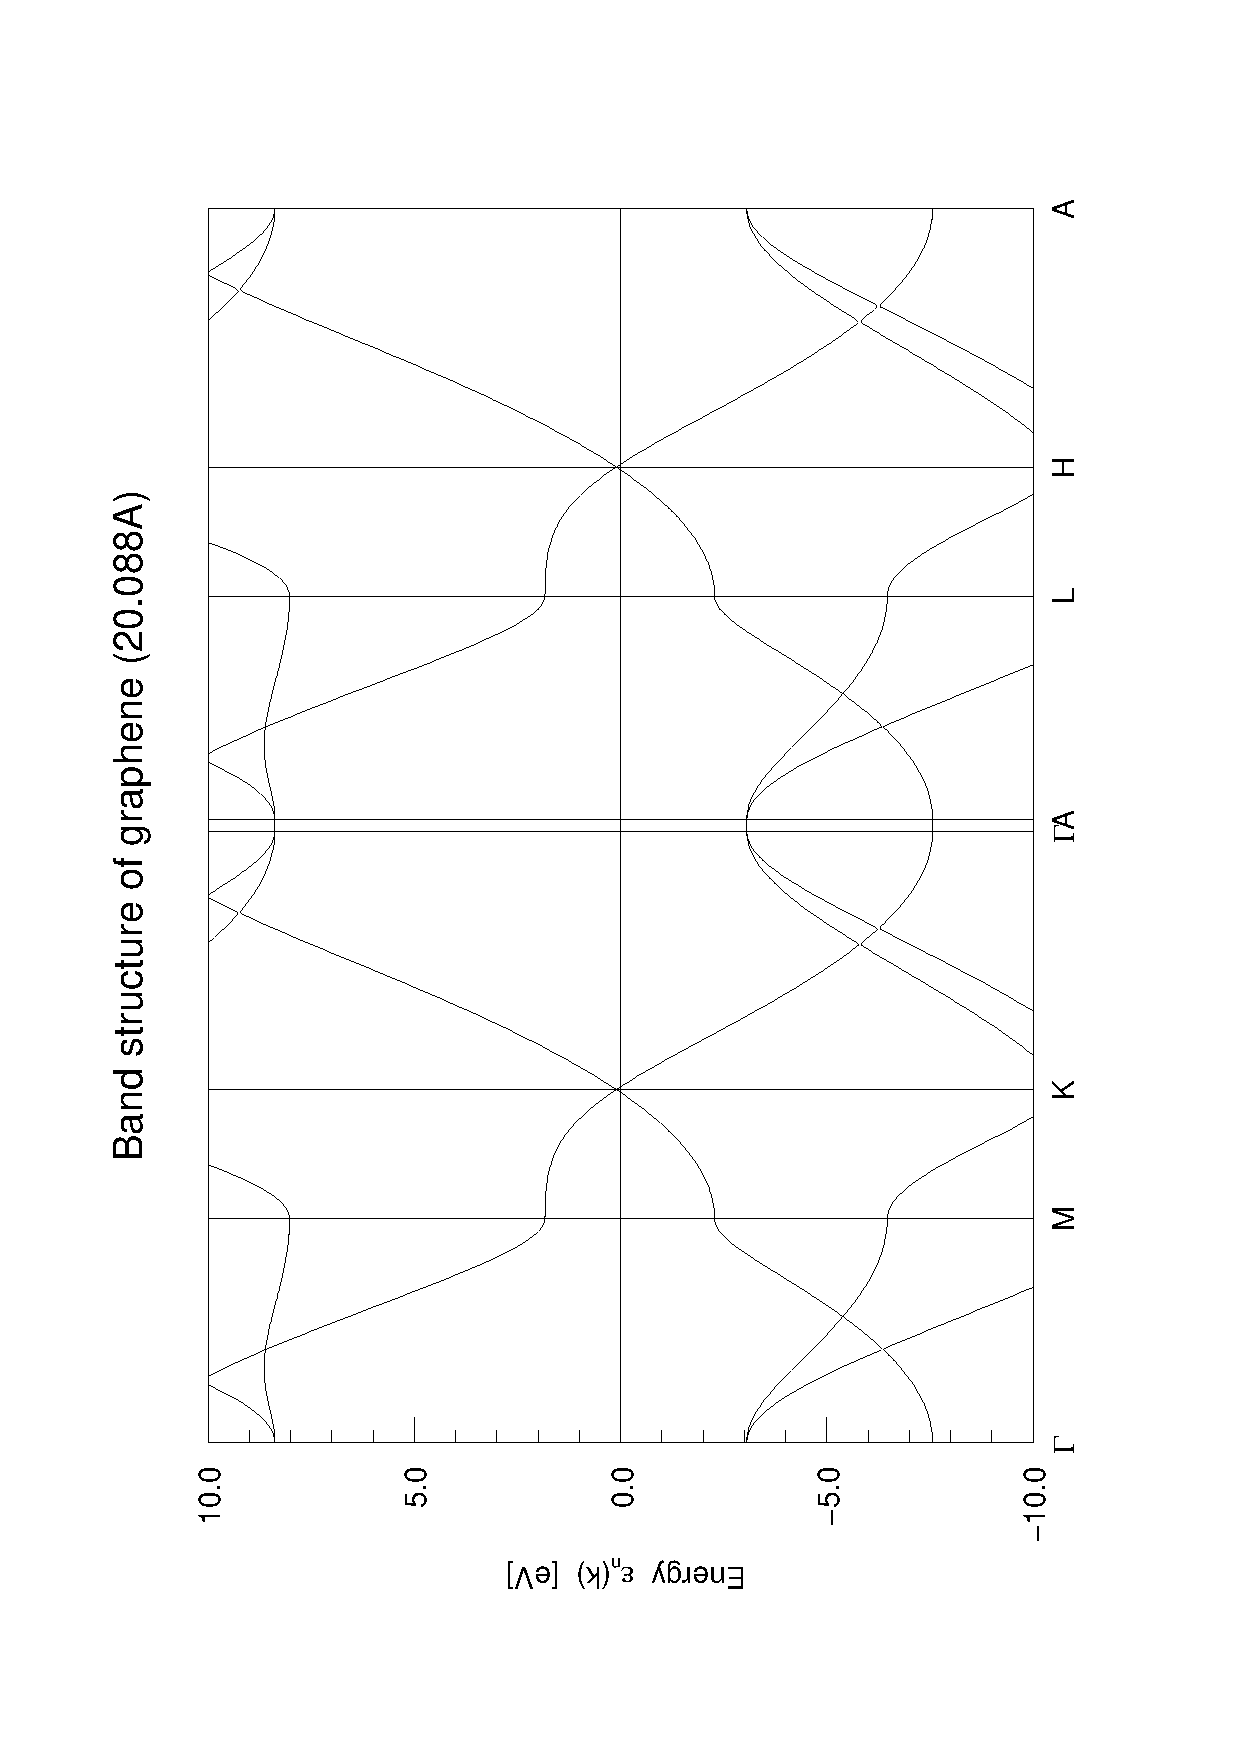
\includegraphics[width=\textwidth]{Results/Graphene/Graphene20A/graphene20Aband.pdf}
					\end{minipage}
					\begin{minipage}[t]{\textwidth}
						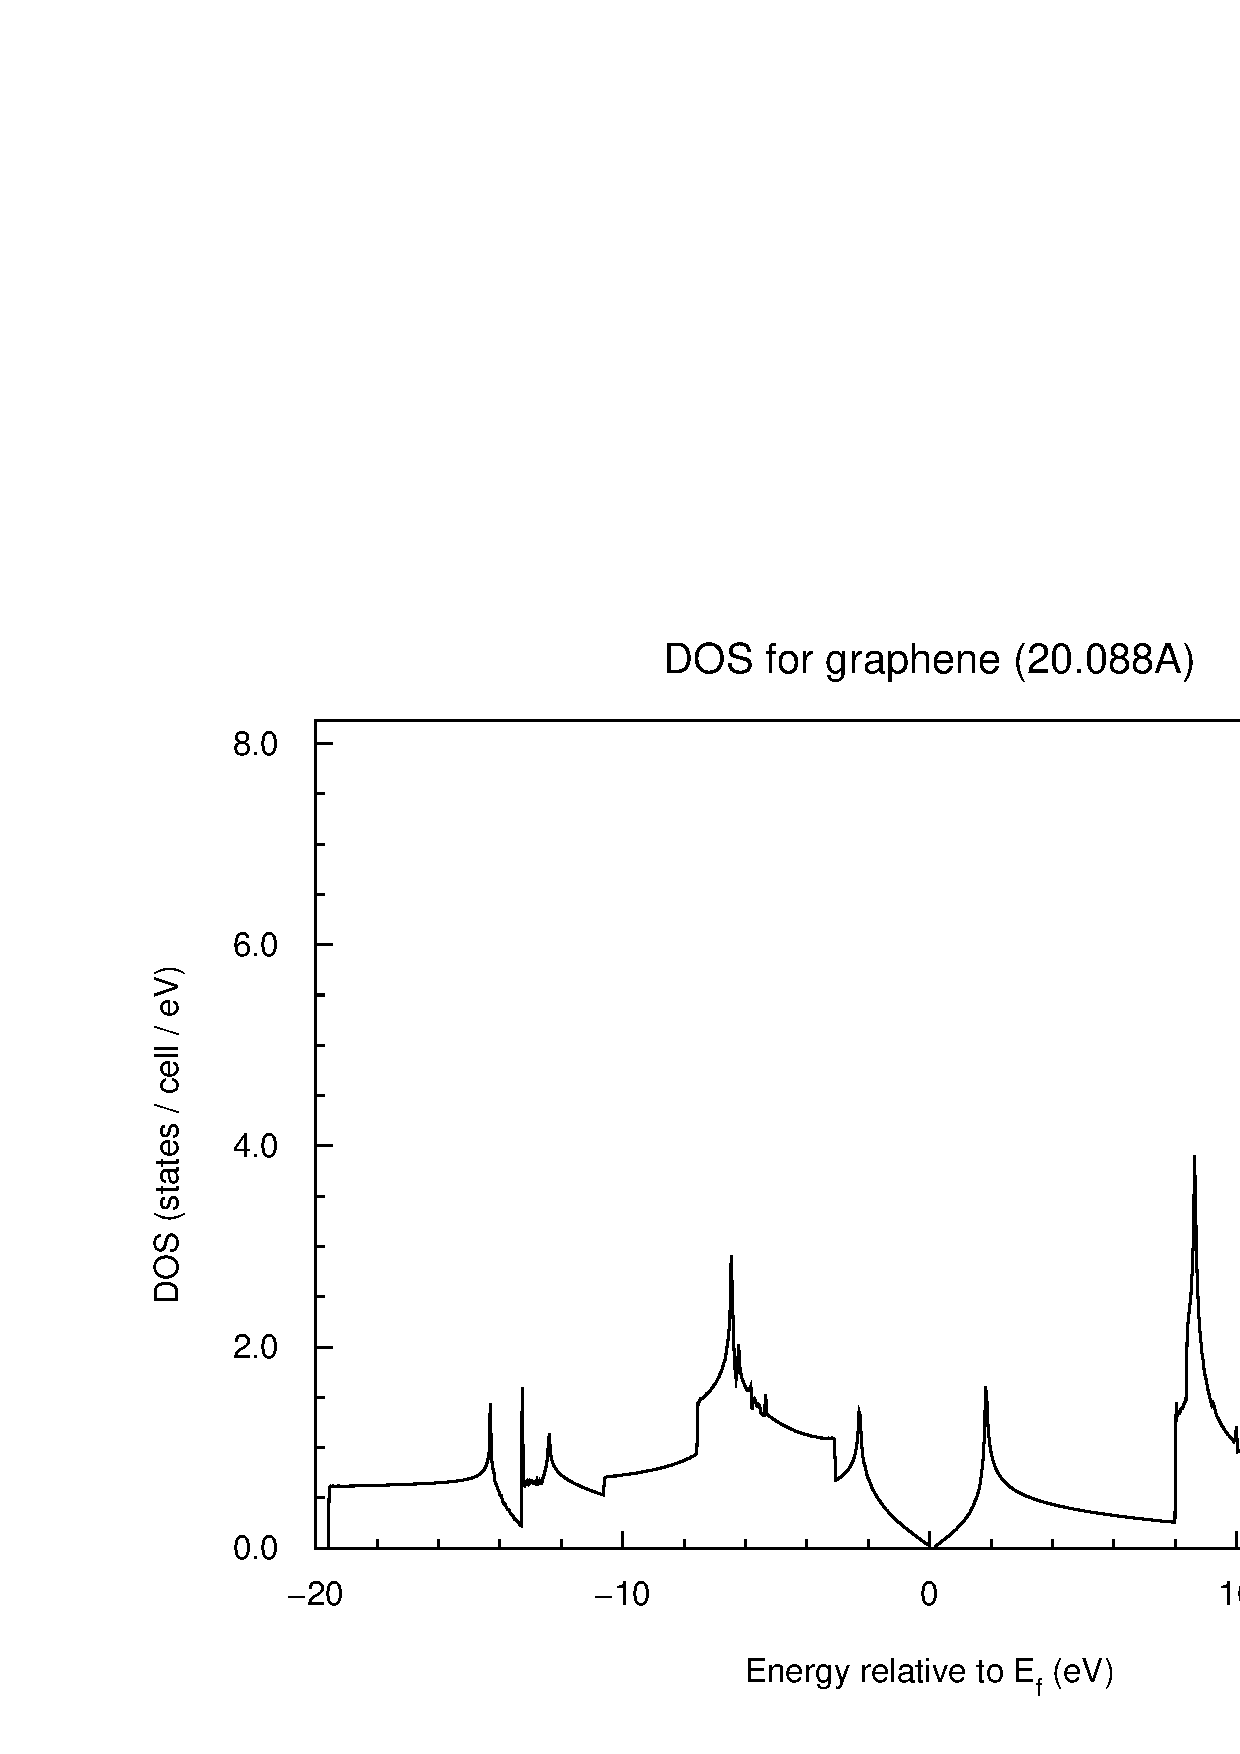
\includegraphics[width=\textwidth]{Results/Graphene/Graphene20A/graphene20Ados.pdf}
					\end{minipage}
					\caption{Band structure and total density of states of graphene (20 $\AA$, FPLO $100\times100\times4$).}
					\label{fig:GrapheneProperties}
				\end{figure}
				\begin{figure}
					\begin{minipage}[t]{\textwidth}
						\includegraphics[width=\textwidth]{Results/Graphene/Graphene20A/graphene20APi.pdf}
					\end{minipage}
					\begin{minipage}[t]{\textwidth}
						\includegraphics[width=\textwidth]{Results/Graphene/Graphene20A/graphene20ASigma.pdf}
					\end{minipage}
					\caption{Weighted band structure of graphene. \textbf{Top:} weighted $\pi$ bands. \textbf{Bottom:} weighted 2s, $2p_x$ and $2p_y$ orbitals. (20 $\AA$, FPLO $100\times100\times4$)}
					\label{fig:GraphenePiSigma}
				\end{figure}
				\begin{figure}
					\includegraphics[width=\textwidth]{Results/Graphene/Graphene20A/graphene20AdosPiSigma.pdf}
					\caption{DOS for the p and sigma-orbitals of graphene with a physically incorrect negative DOS at approximately 18.3 eV (FPLO $100\times100\times4$).}
					\label{fig:GraphenePiSigmaDos}
				\end{figure}				
				Graphene has a total energy of \textbf{-76.168} Ha and three \textbf{sigma} orbitals (2s hybridized with 2p, plotted in Figure \ref{fig:GraphenePiSigma}, bottom), responsible for the planar carbon-carbon bondings and one \textbf{$\pi$} orbital (Figure \ref{fig:GraphenePiSigma}, top). For a whole lattice the $\pi$ orbitals merge and can be seen as delocalized electrons, that are one reason for the copper-equivalent conductivity properties. The contribution of the p and s-orbitals are displayed in Figure \ref{fig:GraphenePiSigmaDos}. We have to mention, that only the $p_z$ orbital contributes to the DOS in the area around the Fermi level. Moreover graphene is a \textbf{zero-gap semiconductor}, i.e. that at the Fermi energy of 0 eV there are no states (Figure \ref{fig:GrapheneProperties}, bottom) and the band-gap is 0 eV. In the band structure (Figure \ref{fig:GrapheneProperties}, top) we find at the K point a 0 eV energy gap, which represents the zero-gap mentioned before and is called \textbf{Dirac point}. At the Dirac point the energy dispersion is linear, which leads to fermions behaving like relativistic particles, described by the Dirac equation near the Dirac point. \\\\
				Before continuing with the modification of graphene we have noticed, that in almost every our DOS plots are physically incorrect negative values. This could be solved by extending the FPLO basis. As a cause we will limited our discussions of areas without significant influence of negative density  of states (Figure \ref{fig:GraphenePiSigmaDos}).
	
			\subsection{Boron-modified graphene}
				\begin{figure}
					\begin{minipage}[t]{\textwidth}
						\includegraphics[width=\textwidth]{Results/Bor/Bor1R/dos.pdf}
					\end{minipage}
					\begin{minipage}[t]{\textwidth}
						\includegraphics[width=\textwidth]{Results/Graphene/GrapheneNew/dos.pdf}
					\end{minipage}		
					\caption{Comparison DOS between boron modified graphene (\textbf{top}, FPLO $20\times20\times20$) and graphene (\textbf{bottom}, FPLO $100\times100\times20$).}
					\label{fig:GrapheneBorDOSComparisson}
				\end{figure}
				\begin{figure}
					\begin{minipage}[t]{\textwidth}
						\includegraphics[width=\textwidth]{Results/Bor/Bor1R/bweights.pdf}
					\end{minipage}
					\begin{minipage}[t]{\textwidth}
						\includegraphics[width=\textwidth]{Results/Graphene/GrapheneNew/bweights.pdf}
					\end{minipage}
					\caption{Comparison of the weighted band structures between boron modified graphene (\textbf{top}, FPLO $20\times20\times20$) and graphene (\textbf{bottom}, FPLO $100\times100\times20$). }
					\label{fig:GrapheneBorBweightsComparisson}
				\end{figure}
				In this section we will discuss the results obtained by different amounts of boron impurities in a graphene lattice. We studied the graphene compound with 50\% of boron impurities. \\\\
				Boron has one valence electron less than carbon and it should therefore lead to an acceptor-intercalated graphene, which means it should increase the electronic conductivity. Regarding the DOS comparison (Figure \ref{fig:GrapheneBorDOSComparisson}) we can conclude that there are more states after the Fermi level in the boron doped lattice, consequently the boron bulk is \textbf{metallic} and the conductivity should be increased. Nevertheless behind the Fermi level opened a gap of approximately 2.6 eV in the DOS, which could limit the conducting properties of the graphene compound. Considering the band structures (Figure \ref{fig:GrapheneBorBweightsComparisson}), we observe the a loss of the Dirac point due to the loss of symmetry. \\\\
				For finding information about the stablest form we tried a relaxation of the given BC mono layer with the FPLO force module, which could not be calculated due too small forces. Therefore we relaxed the lattices manually by fitting the total energy. The only degree of freedom is the lattice parameter in the x and y plane for which we will optimize the total energy. The distance fit (\ref{fig:boronFitting}) yields a optimal parameter of \textbf{2.687} $\boldsymbol{\AA}$ with a total energy of \textbf{-62.881 Ha}.
				\begin{figure}
					\includegraphics[width=\textwidth]{Results/Bor/Bor1R/data.pdf}
					\caption{Distance fitting of $C_{1-x}B_x,x= 1 / 2$.}
					\label{fig:boronFitting}
				\end{figure}
			
			\subsection{Nitrogen modified graphene}
				\begin{figure}
					\begin{minipage}[t]{\textwidth}
						\includegraphics[width=\textwidth]{Results/Nitrogen/Nitrogen1R/bweights.pdf}
					\end{minipage}
					\begin{minipage}[t]{\textwidth}
						\includegraphics[width=\textwidth]{Results/Graphene/GrapheneNew/bweights.pdf}
					\end{minipage}
					\caption{Comparison of the weighted band structures between nitrogen modified graphene (\textbf{top}, FPLO $20\times20\times20$) and graphene (\textbf{bottom}, FPLO $100\times100\times20$).}
					\label{fig:GrapheneNitrogenComparisson}
				\end{figure}
				\begin{figure}
					\begin{minipage}[t]{\textwidth}
						\includegraphics[width=\textwidth]{Results/Nitrogen/Nitrogen1R/dos.pdf}
					\end{minipage}
					\begin{minipage}[t]{\textwidth}
						\includegraphics[width=\textwidth]{Results/Graphene/GrapheneNew/dos.pdf}
					\end{minipage}											
					\caption{Comparison DOS between nitrogen modified graphene (\textbf{top}, FPLO $20\times20\times20$) and graphene (\textbf{bottom}, FPLO $100\times100\times20$).}
					\label{fig:GrapheneNitrogenDOSComparisson}
				\end{figure}
				Having obtained results for boron-doped graphene we want to continue with observing a CN mono-layer. \\\\
				Nitrogen has one valence electron more than carbon and it should therefore lead to a donator-inercalated graphene lattice. As in the boron-carbon compound there are more states near the Fermi level, which implies an improved conductivity. Moreover NC also has a band-gap between -2.6 eV and 7.3 eV. Moreover the NC layer also loses its Dirac point, apparent to the loss of symmetry. \\\\
				\begin{figure}
					\includegraphics[width=\textwidth]{Results/Nitrogen/Nitrogen1R/data.pdf}
					\caption{Unite cell length fit of $C_{1-x}B_x,x= 1 / 2$.}
					\label{fig:nitrogenFitting}
				\end{figure}
				As in Boron doped graphene we now want to focus on the relax the NC compound. Therefore we fitted the energy of different distances (Figure \ref{fig:nitrogenFitting}) and found a minimum at a distance of \textbf{2.477} $\boldsymbol{\AA}$ with an energy of \textbf{-92.743 Ha}.
				
			\subsection{Silicon modified graphene}
				\begin{figure}
					\begin{minipage}[t]{\textwidth}
						\includegraphics[width=\textwidth]{Results/Silicon/Silicon1R/bweights.pdf}
					\end{minipage}
					\begin{minipage}[t]{\textwidth}
						\includegraphics[width=\textwidth]{Results/Graphene/GrapheneNew/bweights.pdf}
					\end{minipage}	
					\caption{Comparison of the weighted band structures between silicon modified graphene (\textbf{top}, FPLO $20\times20\times20$) and graphene (\textbf{bottom}, FPLO $100\times100\times20$).}
					\label{fig:GrapheneSiliconComparisson}
				\end{figure}
				\begin{figure}
					\begin{minipage}[t]{\textwidth}
						\includegraphics[width=\textwidth]{Results/Silicon/Silicon1R/dos.pdf}
					\end{minipage}
					\begin{minipage}[t]{\textwidth}
						\includegraphics[width=\textwidth]{Results/Graphene/GrapheneNew/dos.pdf}
					\end{minipage}											
					\caption{Comparison DOS between silicon modified graphene (\textbf{top}, FPLO $20\times20\times20$) and graphene (\textbf{bottom}, FPLO $100\times100\times20$).}
					\label{fig:GrapheneSiliconDOSComparisson}
				\end{figure}
				The last material we want to observe is silicon doped graphene. Silicon is in the same group as carbon, i.e. its count of valence electrons is equal to carbon. On he other hand it is located in the next period hence it has plenty more electrons and a bigger atomic radius than boron or nitrogen. Due to the many electrons the Fermi level and the orbitals previously responsible for the electronic properties changed from 2s and 2p to 3s and 3p (Figure \ref{fig:GrapheneSiliconComparisson}). In Addition the SC mono layer has a band gap of approximated 2 eV and is therefore a semiconductor. Nevertheless it has a very high state of density right before the Fermi level. \\\\
				\begin{figure}
					\includegraphics[width=\textwidth]{Results/Silicon/Silicon1R/data.pdf}
					\caption{Distance fitting of $C_{1-x}B_x,x= 1 / 2$.}
					\label{fig:siliconFitting}
				\end{figure}
				For a observation of the stability we found the energetic minimum at a unit cell length of \textbf{3.112} $\boldsymbol{\AA}$, which leads to the biggest unit cell size of all three compounds, caused presumable due to the huge atom radius of silicon ($\approx 111$ pm).
				In Addition the total energy of the silicon compound is very different to the total energy of nitrogen or boron with a value of \textbf{-327.459 eV}.
				\begin{table}[H]
					\centering
					\begin{tabular}{cccc}
						\midrule
						C & B & N & Si \\
						\midrule 
						-76.168 eV & -62.881 Ha & -92.743 Ha & -327.459 Ha \\
						\bottomrule
					\end{tabular}
					\caption{Comparison of the total energy's for graphene and graphene modified with boron, nitrogen or silicon.}
				\end{table}
				\begin{table}[H]
					\centering
					\begin{tabular}{cccc}
						\midrule
						C & B & N & Si \\
						\midrule 
						2.456 $\AA$ & 2.687 $\AA$ & 2.477 $\AA$ & 3.112 $\AA$ \\
						\bottomrule
					\end{tabular}
					\caption{Comparison of graphene and the relaxed unite cell lengths.}
				\end{table}				
				For the purpose of completeness we added band structures and density of states of different modifications and doping densities (see Figures \ref{fig:BoronDensityComparisson}, \ref{fig:NitrogenDensityComparisson}, \ref{fig:SiliconDensityComparisson}, \ref{fig:BoronDOSDensityComparisson}, \ref{fig:NitrogenDOSComparisson}, \ref{fig:SiliconDOSComparisson}). From the figures we can obtain, that the number of bands rise with the size of the unite cell, caused by the number of unequal atoms, having different orbitals. Furthermore we obtain for a reducing density a rising graphene character by comparing the density of states.
				\begin{figure}
					\begin{minipage}[t]{0.9\textwidth}
						\includegraphics[width=\textwidth]{Results/Bor/Bor1/bor1band.pdf}
					\end{minipage}
					\begin{minipage}[t]{0.9\textwidth}
						\includegraphics[width=\textwidth]{Results/Bor/Bor5/bor5band.pdf}
					\end{minipage}
					\begin{minipage}[t]{0.3\textwidth}
						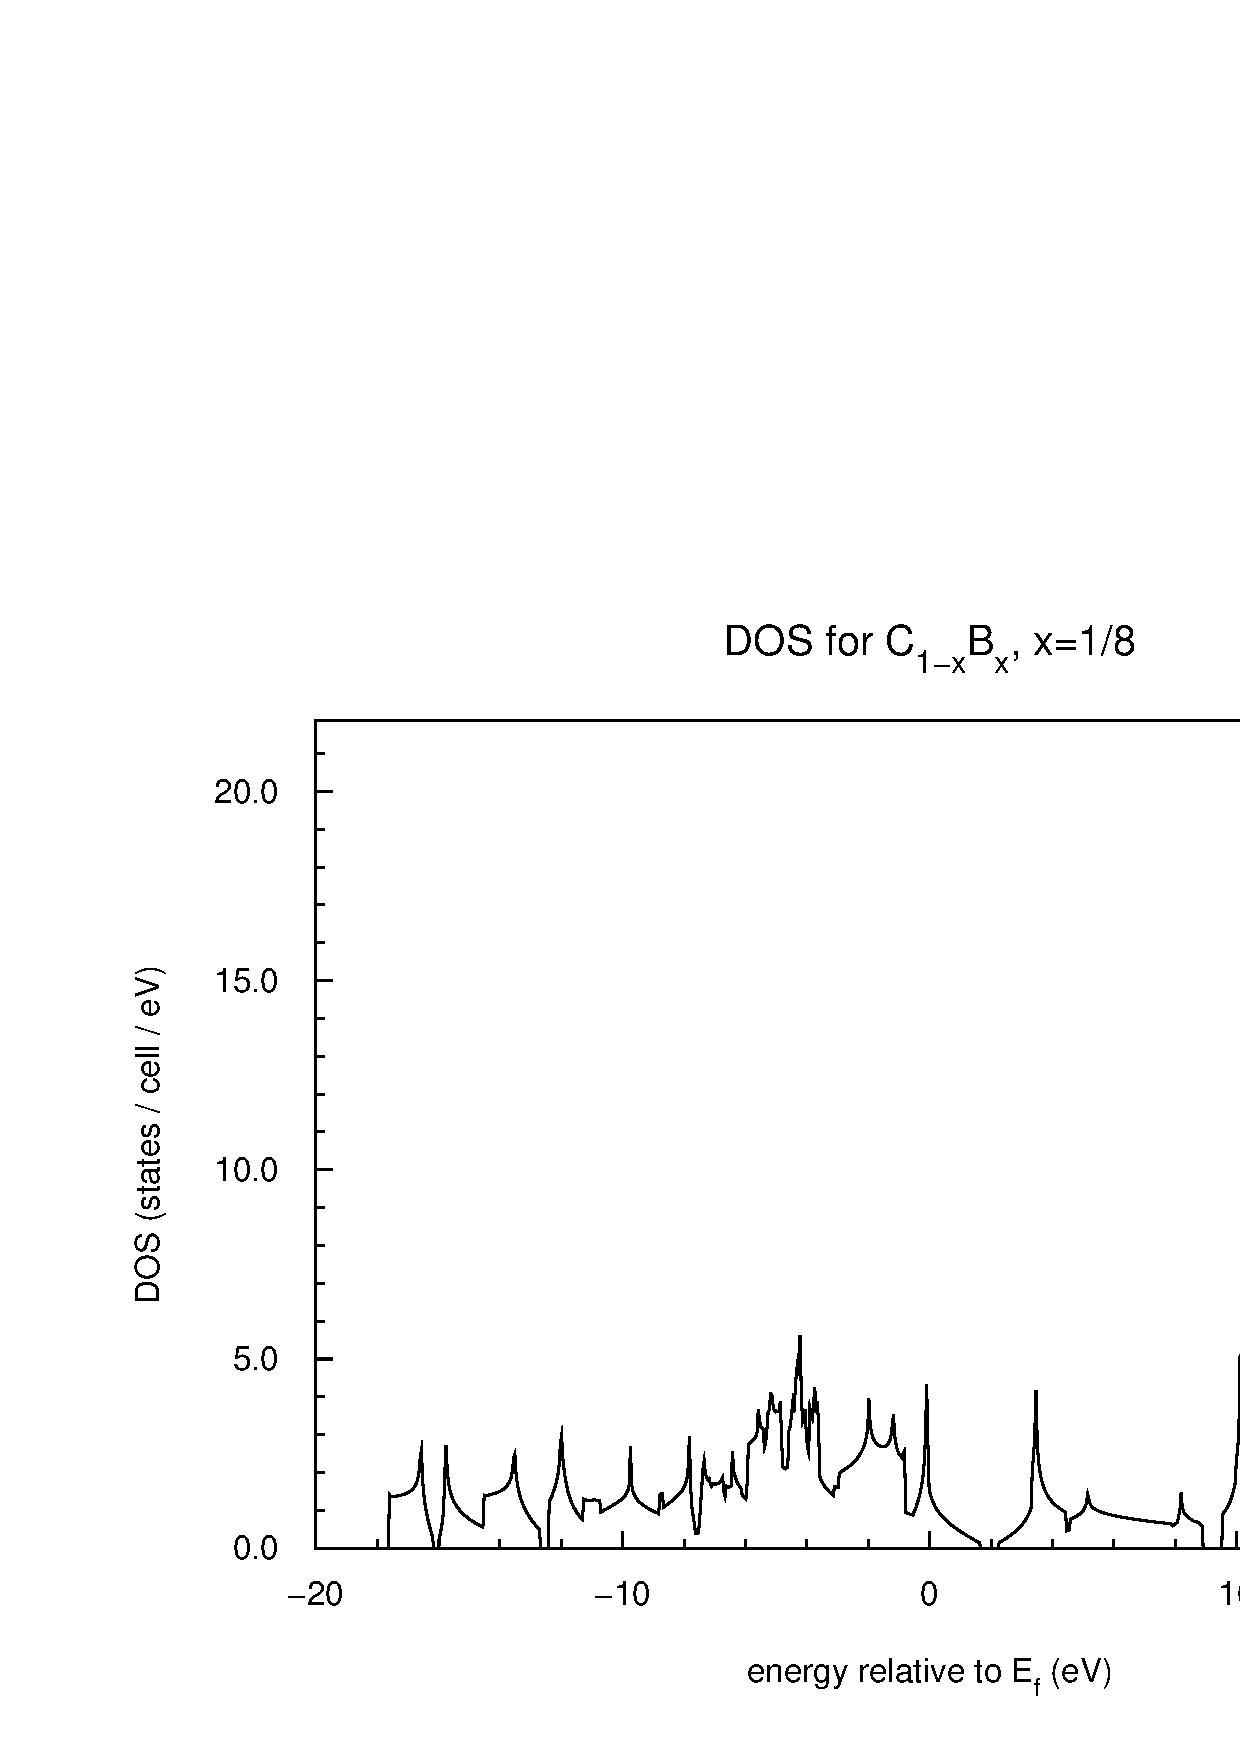
\includegraphics[width=\textwidth]{Results/Bor/Bor2/bor2band.pdf}
					\end{minipage}
					\begin{minipage}[t]{0.3\textwidth}
						\includegraphics[width=\textwidth]{Results/Bor/Bor3/bor3band.pdf}
					\end{minipage}
					\begin{minipage}[t]{0.3\textwidth}
						\includegraphics[width=\textwidth]{Results/Bor/Bor4/bor4band.pdf}
					\end{minipage}															
					\caption{Comparison of the band structures from boron-modified graphene with different densities (FPLO $100x100x4$).}
					\label{fig:BoronDensityComparisson}
				\end{figure}				
				\begin{figure}
					\begin{minipage}[t]{0.9\textwidth}
						\includegraphics[width=\textwidth]{Results/Nitrogen/Nitrogen1/nitrogen1band.pdf}
					\end{minipage}
					\begin{minipage}[t]{0.9\textwidth}
						\includegraphics[width=\textwidth]{Results/Nitrogen/Nitrogen5/nitrogen5band.pdf}
					\end{minipage}
					\begin{minipage}[t]{0.3\textwidth}
						\includegraphics[width=\textwidth]{Results/Nitrogen/Nitrogen2/nitrogen2band.pdf}
					\end{minipage}
					\begin{minipage}[t]{0.3\textwidth}
						\includegraphics[width=\textwidth]{Results/Nitrogen/Nitrogen3/nitrogen3band.pdf}
					\end{minipage}
					\begin{minipage}[t]{0.3\textwidth}
						\includegraphics[width=\textwidth]{Results/Nitrogen/Nitrogen4/nitrogen4band.pdf}
					\end{minipage}															
					\caption{Comparison of the band structures from nitrogen-modified graphene with different densities (FPLO $100x100x4$)}
					\label{fig:NitrogenDensityComparisson}
				\end{figure}
				\begin{figure}
					\begin{minipage}[t]{0.9\textwidth}
						\includegraphics[width=\textwidth]{Results/Silicon/Silicon1/silicon1band.pdf}
					\end{minipage}
					\begin{minipage}[t]{0.9\textwidth}

						\includegraphics[width=\textwidth]{Results/Silicon/Silicon5/silicon5band.pdf}
					\end{minipage}
					\begin{minipage}[t]{0.3\textwidth}
						\includegraphics[width=\textwidth]{Results/Silicon/Silicon2/silicon2band.pdf}
					\end{minipage}
					\begin{minipage}[t]{0.3\textwidth}
						\includegraphics[width=\textwidth]{Results/Silicon/Silicon3/silicon3band.pdf}
					\end{minipage}
					\begin{minipage}[t]{0.3\textwidth}
						\includegraphics[width=\textwidth]{Results/Silicon/Silicon4/silicon4band.pdf}
					\end{minipage}															
					\caption{Comparison of the band structures from silicon-modified graphene with different densities (FPLO $100x100x4$)}
					\label{fig:SiliconDensityComparisson}
				\end{figure}
				\begin{figure}
					\begin{minipage}[t]{0.9\textwidth}
						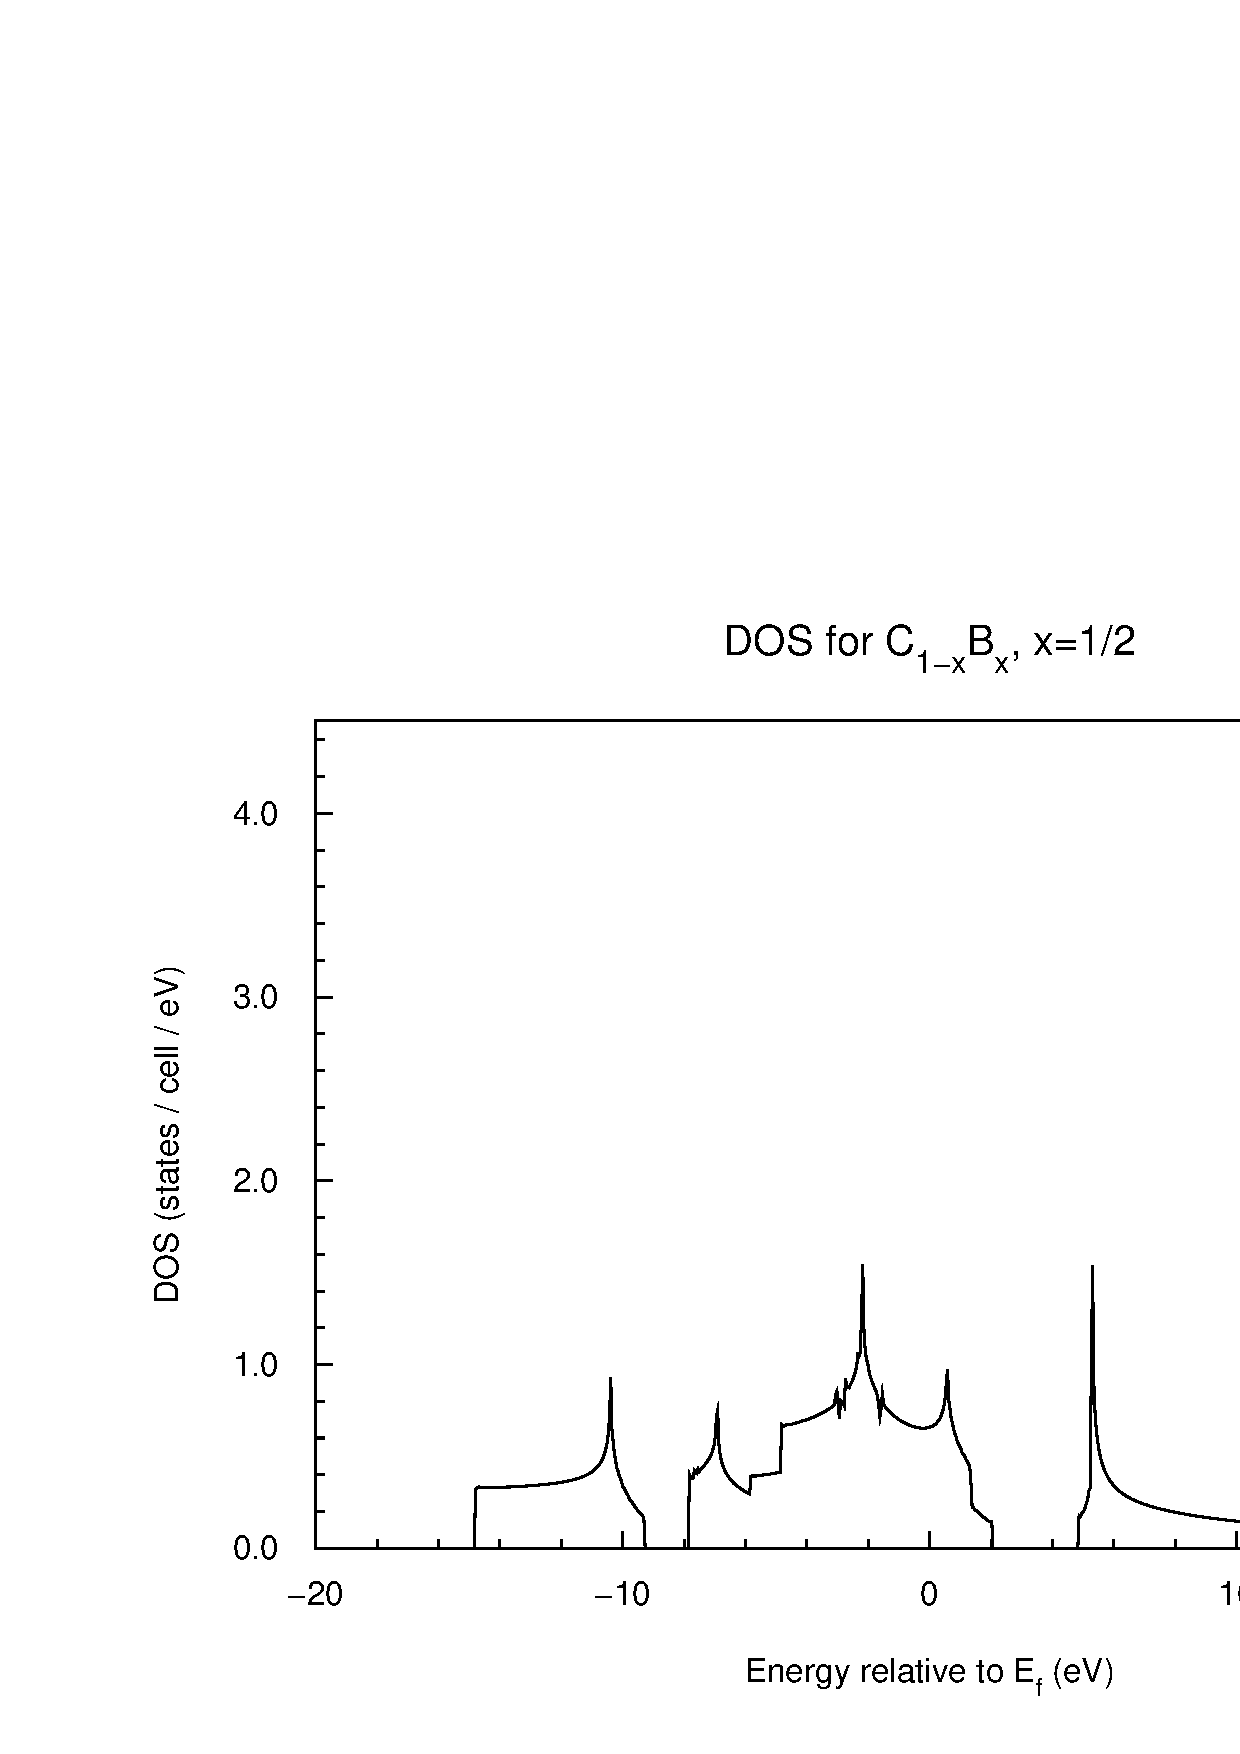
\includegraphics[width=\textwidth]{Results/Bor/Bor1/bor1dos.pdf}
					\end{minipage}
					\begin{minipage}[t]{0.9\textwidth}
						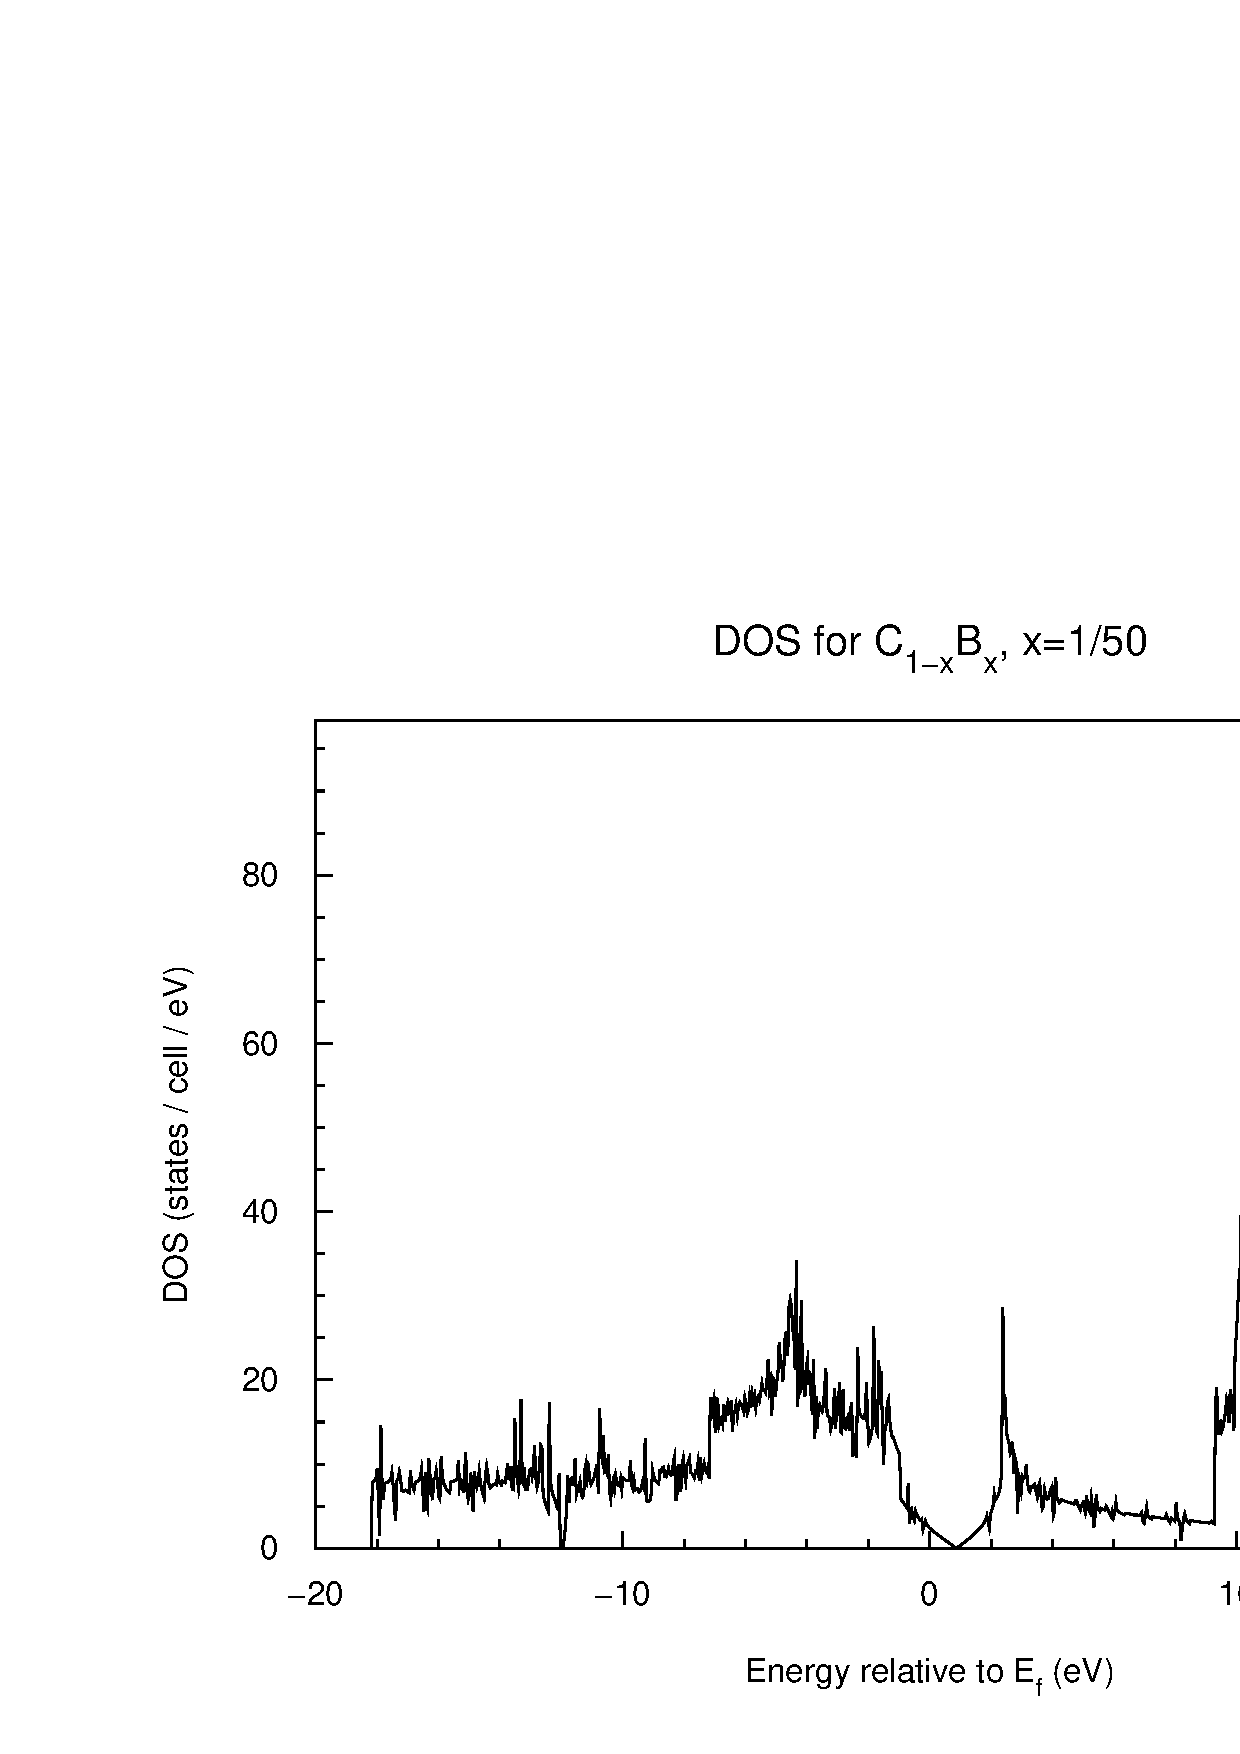
\includegraphics[width=\textwidth]{Results/Bor/Bor5/bor5dos.pdf}
					\end{minipage}
					\begin{minipage}[t]{0.3\textwidth}
						\includegraphics[width=\textwidth]{Results/Bor/Bor2/bor2dos.pdf}
					\end{minipage}
					\begin{minipage}[t]{0.3\textwidth}
						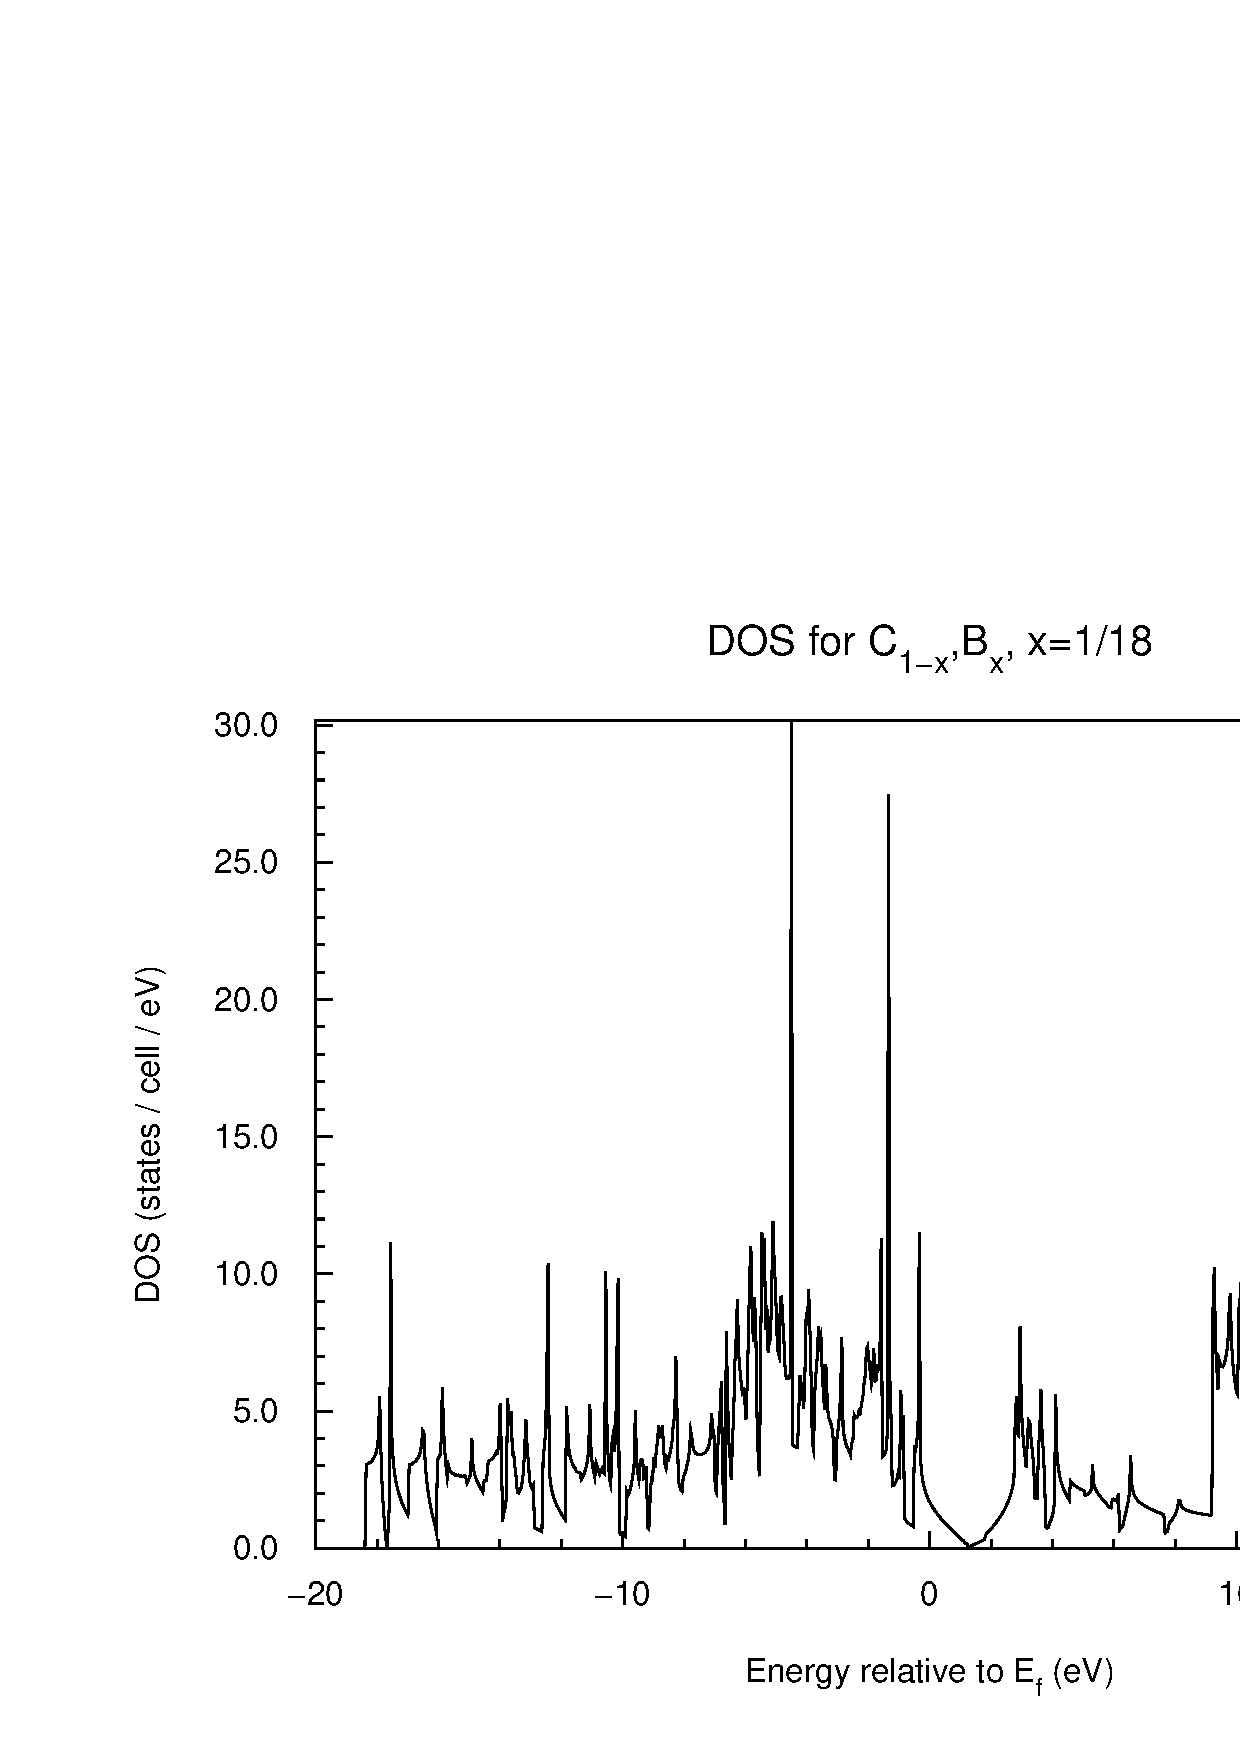
\includegraphics[width=\textwidth]{Results/Bor/Bor3/bor3dos.pdf}
					\end{minipage}
					\begin{minipage}[t]{0.3\textwidth}
						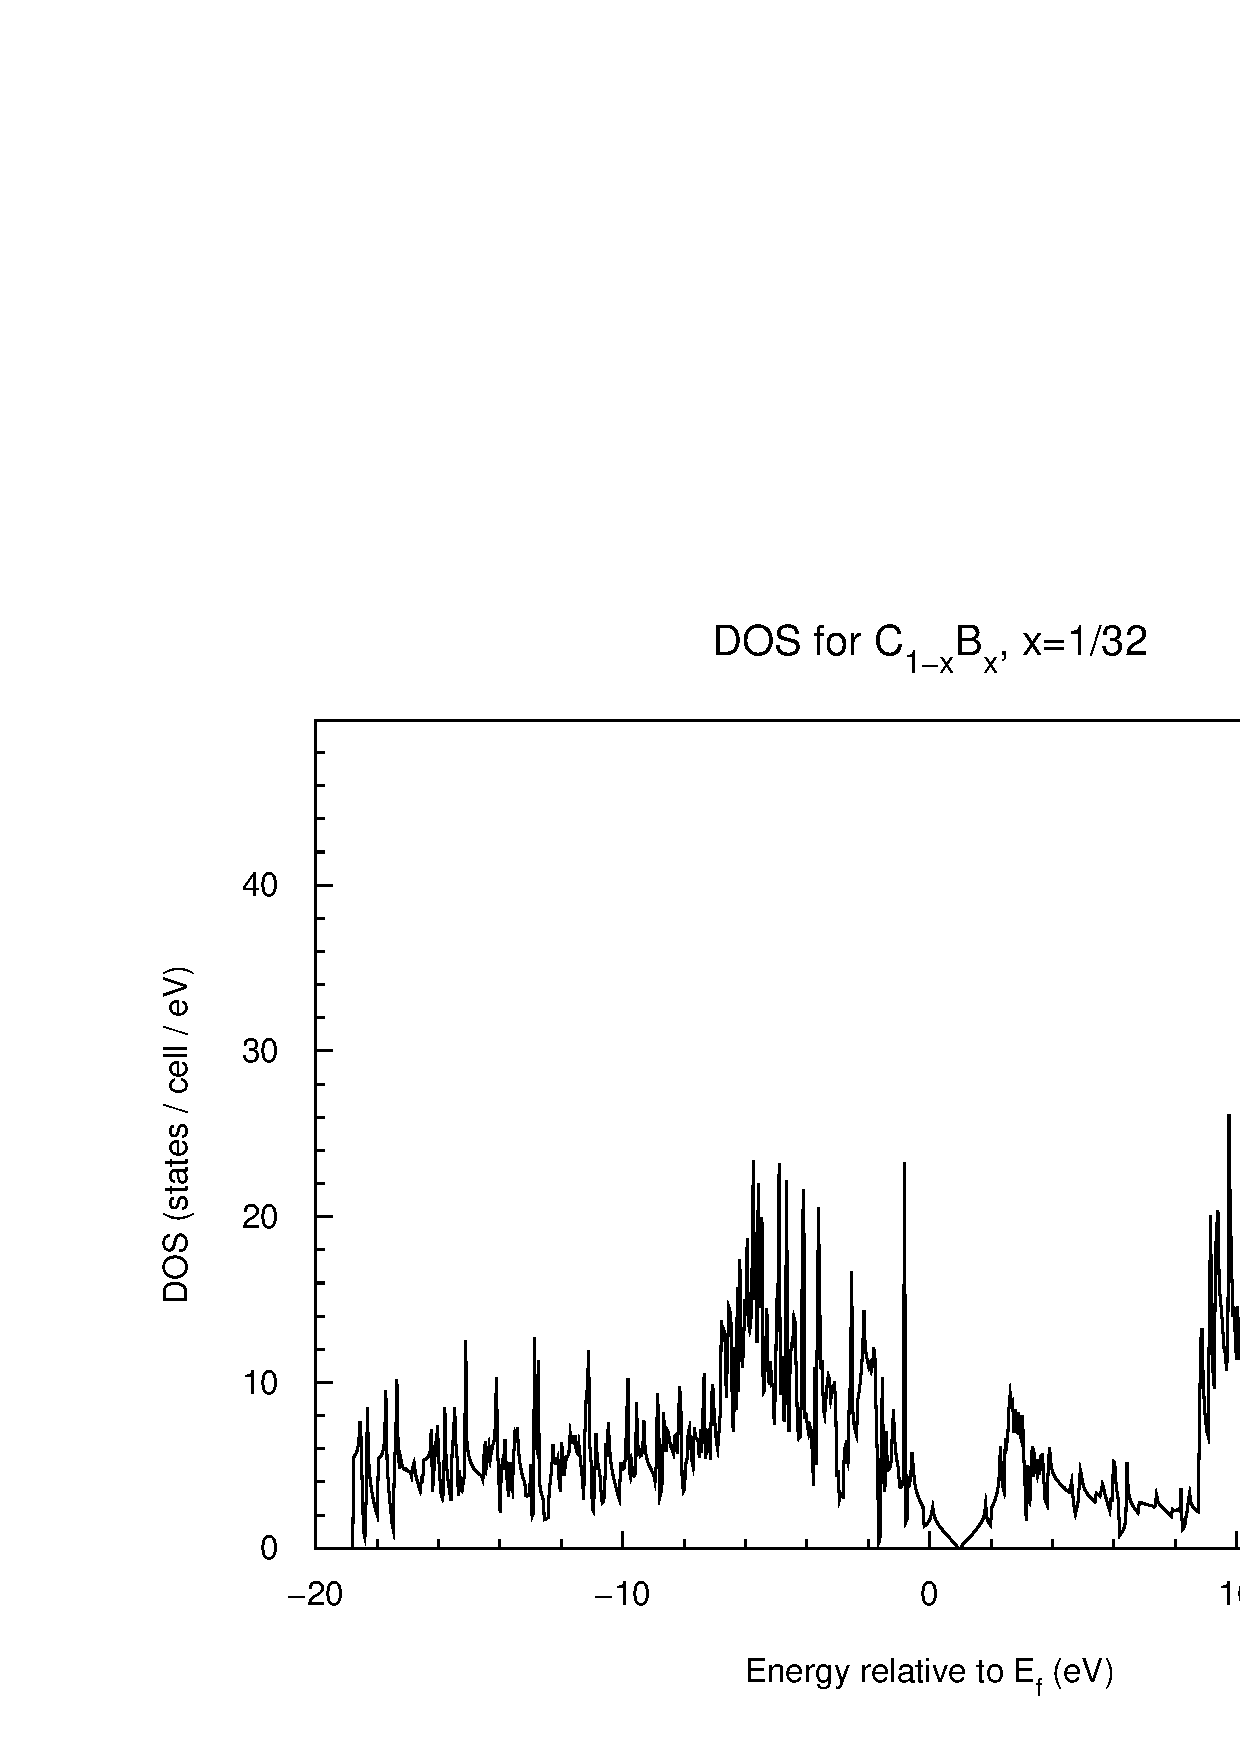
\includegraphics[width=\textwidth]{Results/Bor/Bor4/bor4dos.pdf}
					\end{minipage}															
					\caption{Comparison of the DOS from boron-modified graphene with different densities (FPLO $100x100x4$)}
					\label{fig:BoronDOSDensityComparisson}
				\end{figure}				
				\begin{figure}
					\begin{minipage}[t]{0.9\textwidth}
						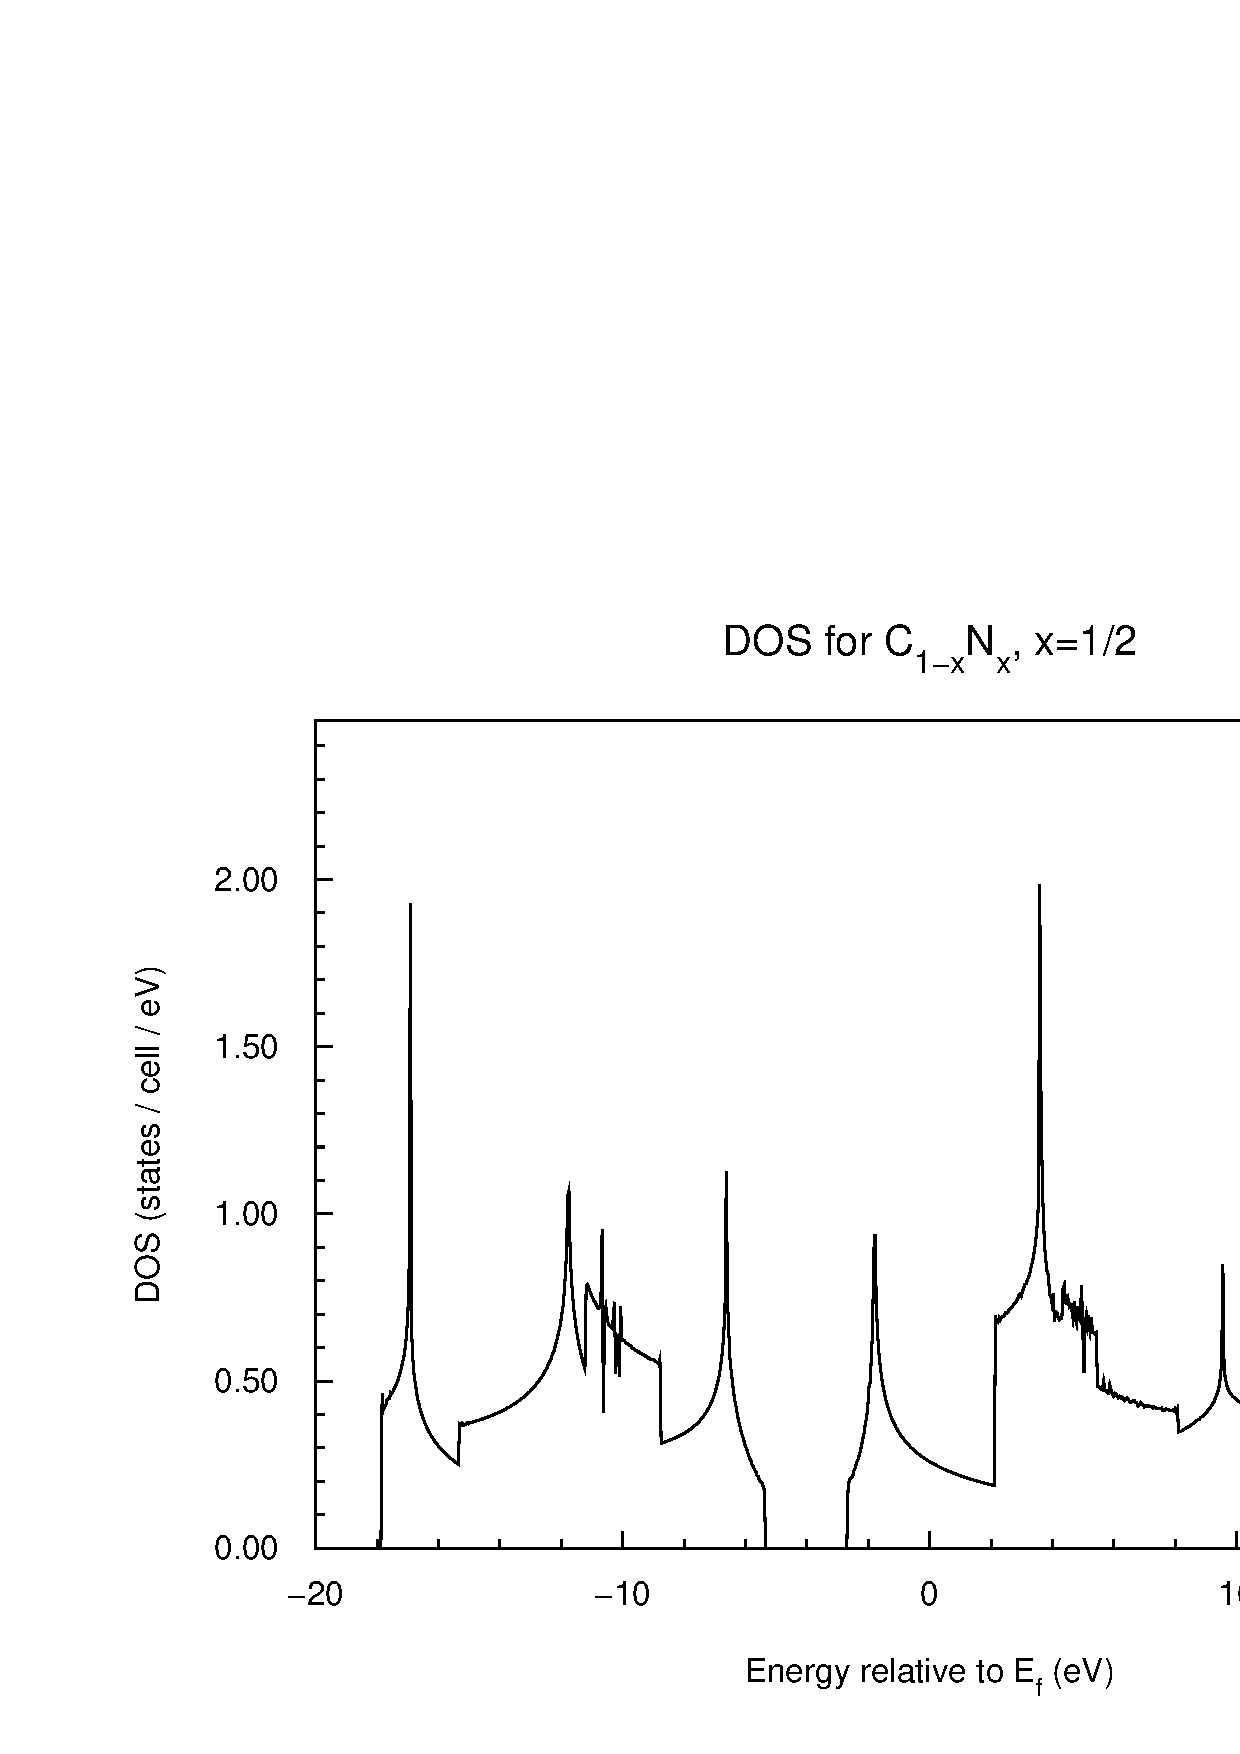
\includegraphics[width=\textwidth]{Results/Nitrogen/Nitrogen1/nitrogen1dos.pdf}
					\end{minipage}
					\begin{minipage}[t]{0.9\textwidth}
						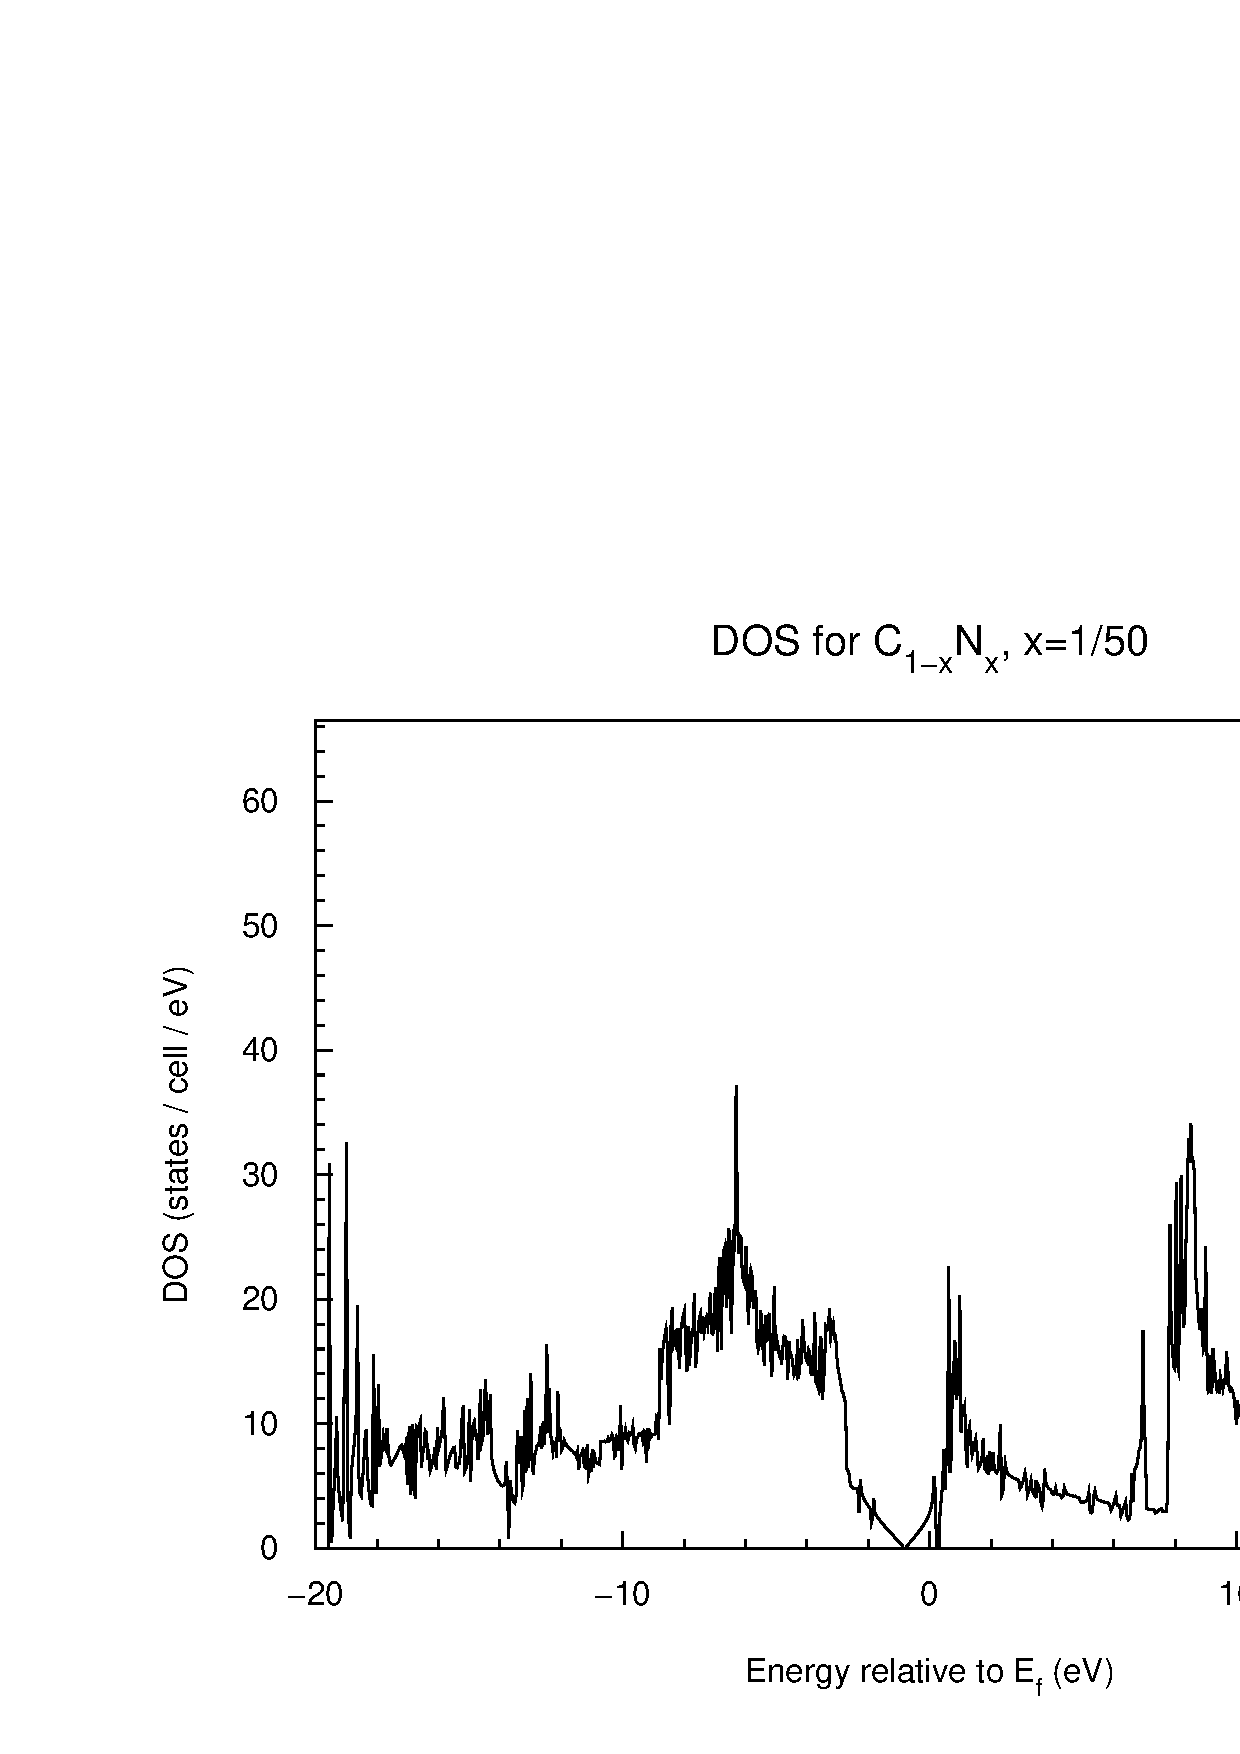
\includegraphics[width=\textwidth]{Results/Nitrogen/Nitrogen5/nitrogen5dos.pdf}
					\end{minipage}
					\begin{minipage}[t]{0.3\textwidth}
						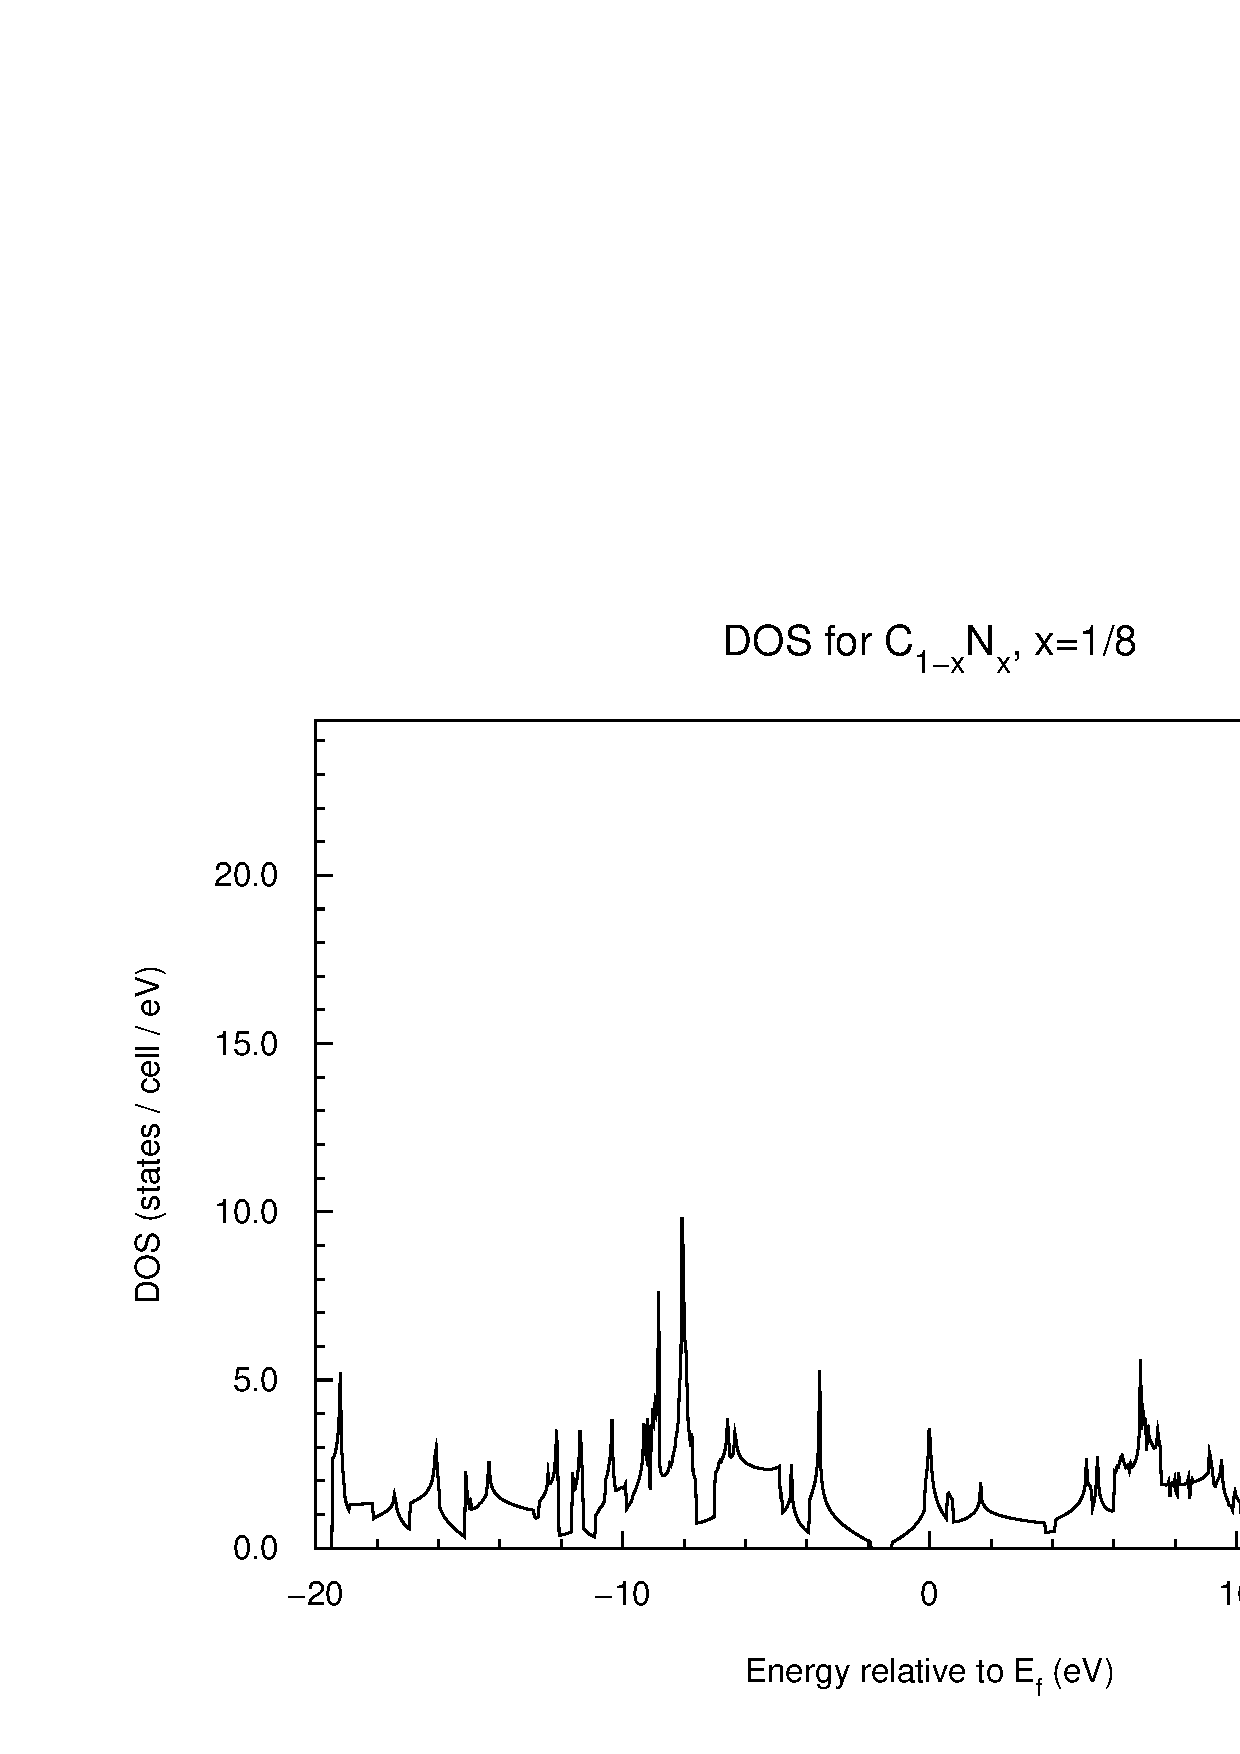
\includegraphics[width=\textwidth]{Results/Nitrogen/Nitrogen2/nitrogen2dos.pdf}
					\end{minipage}
					\begin{minipage}[t]{0.3\textwidth}
						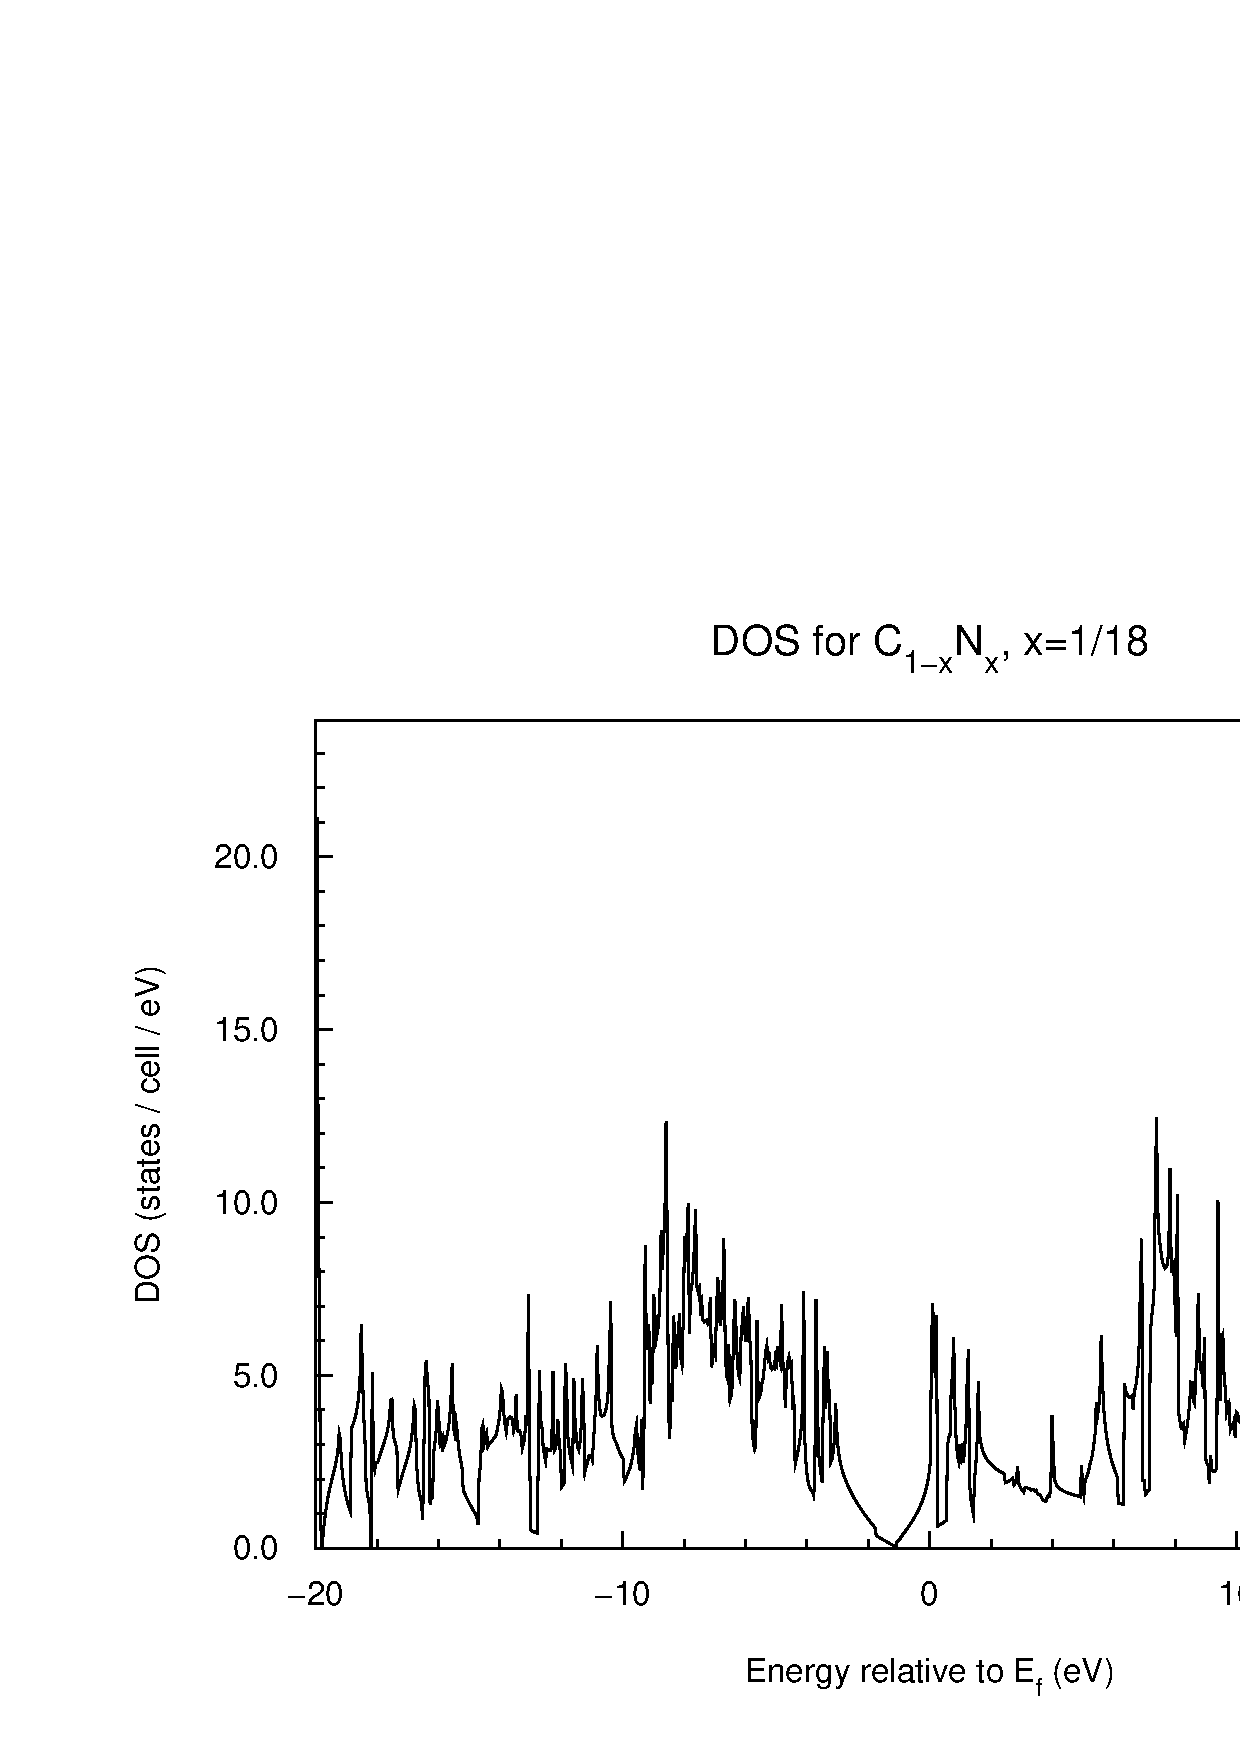
\includegraphics[width=\textwidth]{Results/Nitrogen/Nitrogen3/nitrogen3dos.pdf}
					\end{minipage}
					\begin{minipage}[t]{0.3\textwidth}
						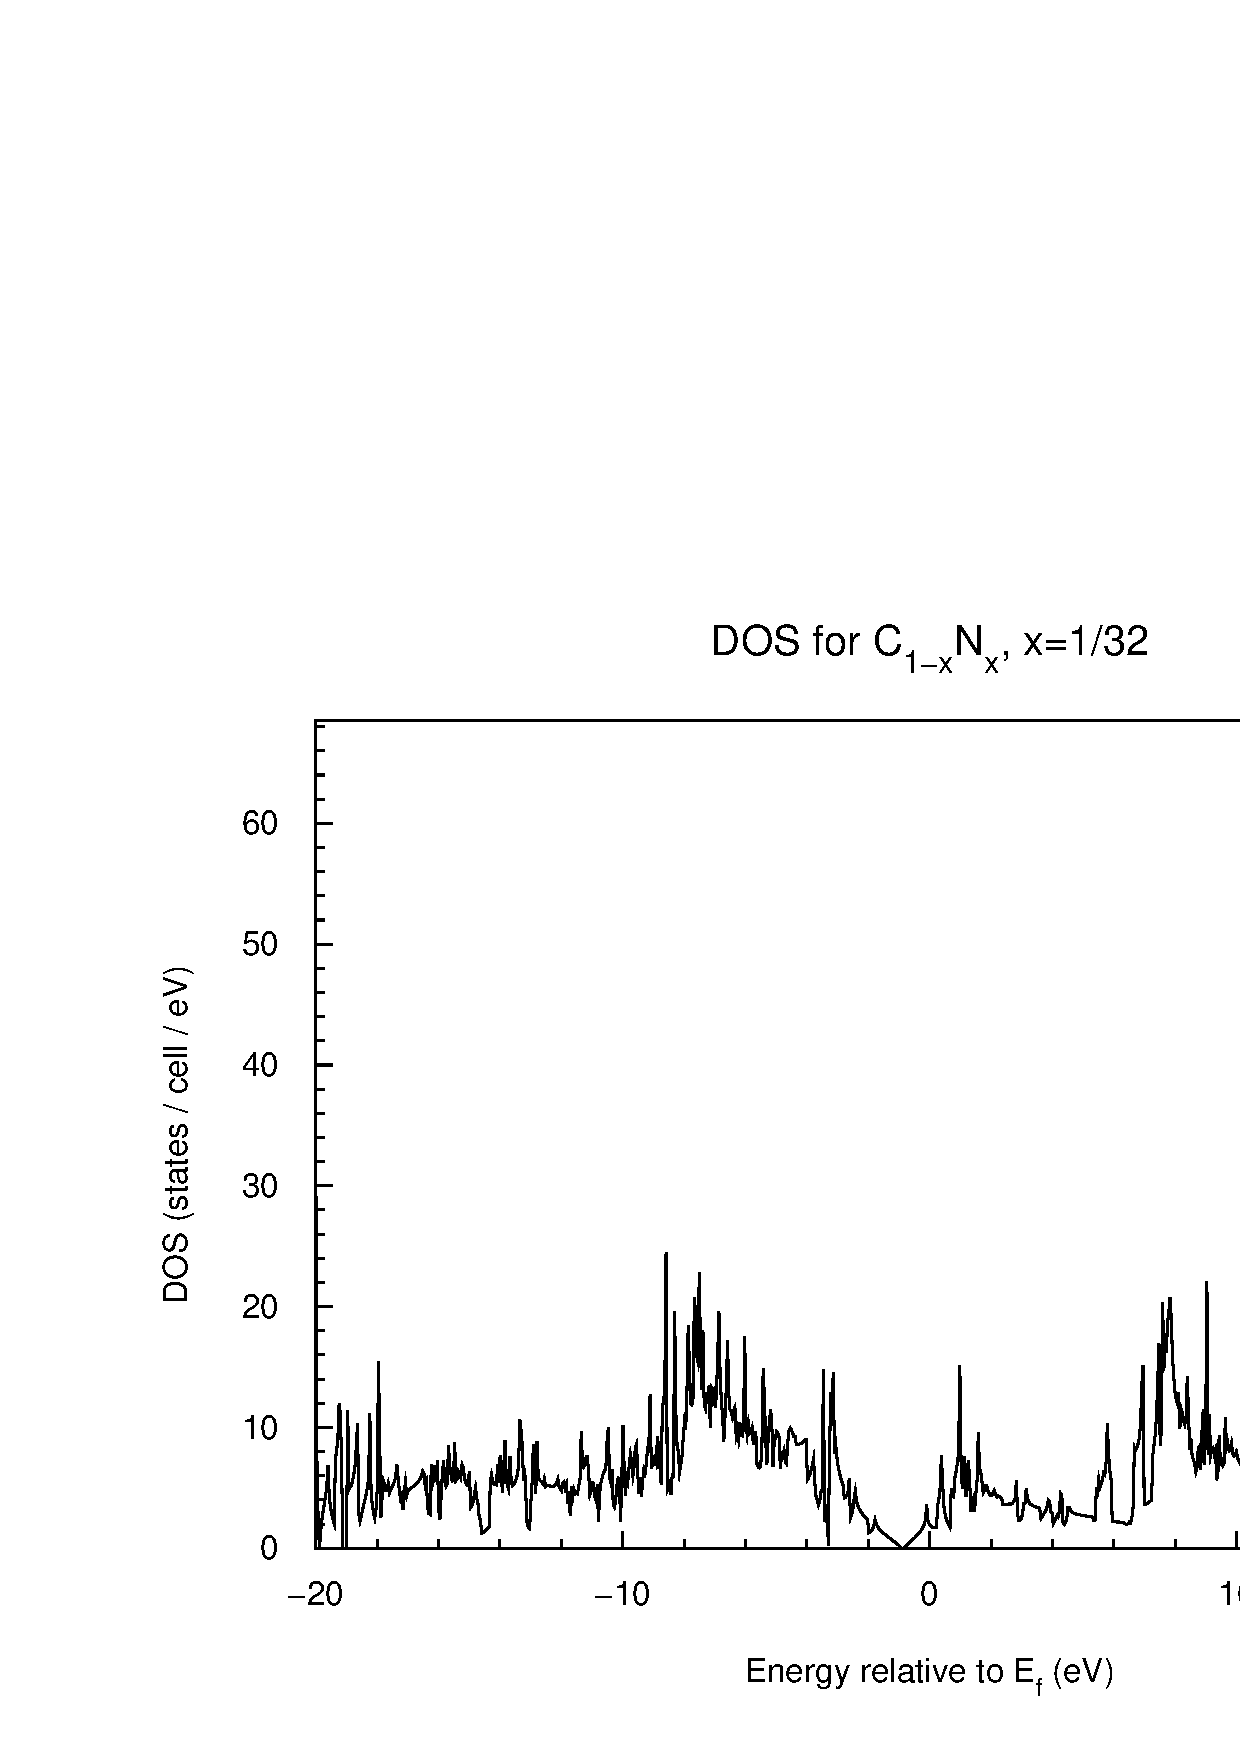
\includegraphics[width=\textwidth]{Results/Nitrogen/Nitrogen4/nitrogen4dos.pdf}
					\end{minipage}															
					\caption{Comparison of the DOS from nitrogen-modified graphene with different densities (FPLO $100x100x4$)}
					\label{fig:NitrogenDOSComparisson}
				\end{figure}
				\begin{figure}
					\begin{minipage}[t]{0.9\textwidth}
						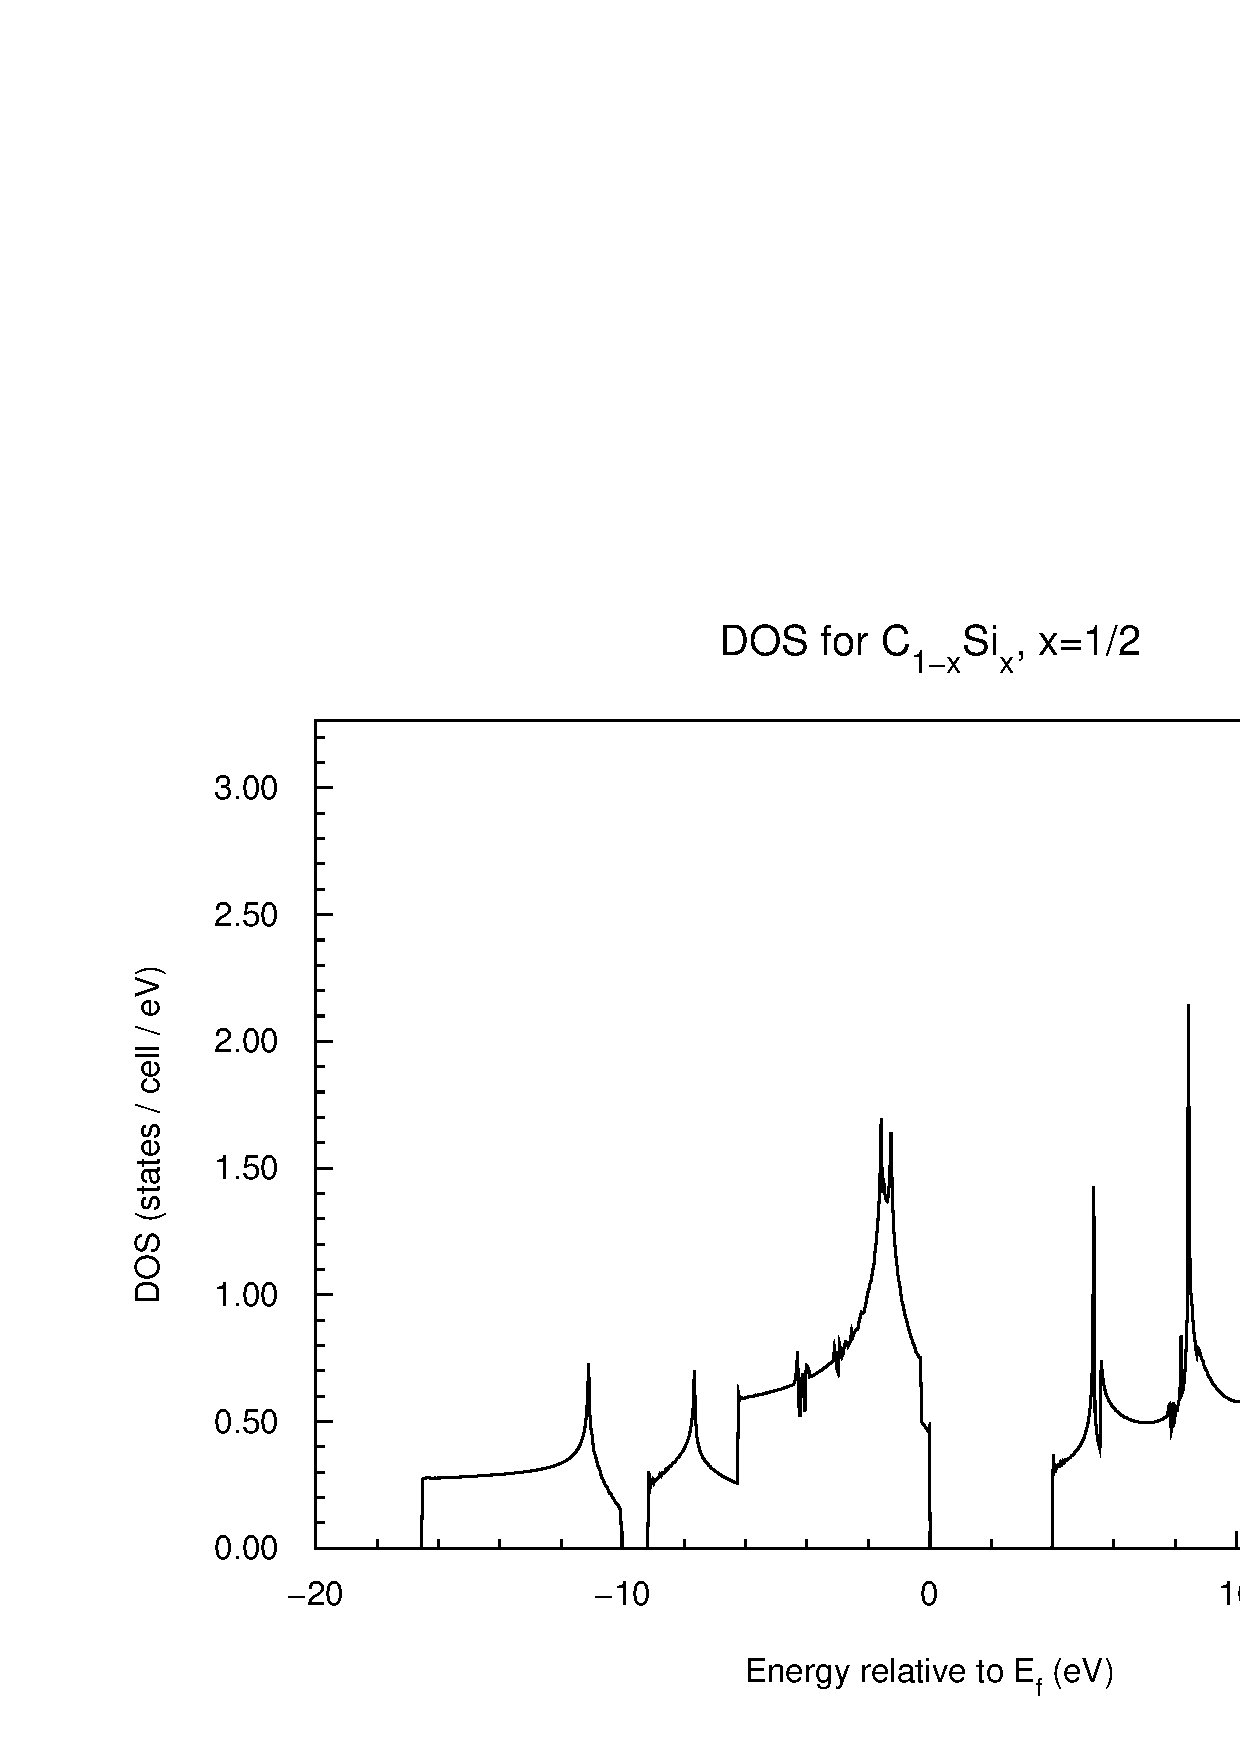
\includegraphics[width=\textwidth]{Results/Silicon/Silicon1/silicon1dos.pdf}
					\end{minipage}
					\begin{minipage}[t]{0.9\textwidth}
						\includegraphics[width=\textwidth]{Results/Silicon/Silicon5/silicon5dos.pdf}
					\end{minipage}
					\begin{minipage}[t]{0.3\textwidth}
						\includegraphics[width=\textwidth]{Results/Silicon/Silicon2/silicon2dos.pdf}
					\end{minipage}
					\begin{minipage}[t]{0.3\textwidth}
						\includegraphics[width=\textwidth]{Results/Silicon/Silicon3/silicon3dos.pdf}
					\end{minipage}
					\begin{minipage}[t]{0.3\textwidth}
						\includegraphics[width=\textwidth]{Results/Silicon/Silicon4/silicon4dos.pdf}
					\end{minipage}															
					\caption{Comparison of the DOS from silicon-modified graphene with different densities (FPLO $100x100x4$)}
					\label{fig:SiliconDOSComparisson}
				\end{figure}
				
				
					
				
				

				
			
	
	
			
		
		
		
			
		
		
		
		
		
		
		
			 
		
		

		